\documentclass[12pt,oneside,a4paper]{book} % This style for A4 format.

%Packages
\usepackage{ecproject}
\usepackage{graphicx}
\usepackage{tikz}
\usetikzlibrary{calc}
\usepackage[a4paper, margin=1in]{geometry}
\usepackage{float}
\usepackage{qrcode}
%%%Page related
\usepackage{fancyhdr} % for header & footer
\usepackage[hidelinks]{hyperref}
\usepackage[toc, nonumberlist]{glossaries} %For Glossaries - to be loaded only after hyperref package
%\usepackage[automake]{glossaries-extra}
% For code snippets
\usepackage[listings]{tcolorbox}
    \tcbuselibrary{skins,breakable}
    \tcbuselibrary{theorems}
%\ifIndentPara
\usepackage{indentfirst}
%\fi
\usepackage{setspace}
%%%Table Related
%\usepackage{booktabs}
%\usepackage{makecell}
%\usepackage{multirow}
%\usepackage{multicol}

% TikZ and its libraries
\usepackage{tikz}
\usetikzlibrary{shapes, arrows.meta, positioning, calc, circuits.ee.IEC}

% PGFPlots and its libraries
\usepackage{pgfplots}
\usepgfplotslibrary{fillbetween}
\pgfplotsset{compat=1.18}

% Math and Symbols
\usepackage{amsmath}
\usepackage{pifont}   % for \ding{51} checkmark and \ding{55} cross
\usepackage{tikz}
\usepackage{pgfplots}
\pgfplotsset{compat=1.18}
\usetikzlibrary{shapes,arrows.meta,positioning,calc,fillbetween}
\usepackage{amsmath}
\usepackage{pifont}   % for \ding{51} checkmark and \ding{55} cross
\usepackage{pgfplots}
\pgfplotsset{compat=1.18}
\usetikzlibrary{shapes,arrows.meta,positioning,calc}
%%%%%%%%%%%%%%%%%%%%%%%%%%%%%%%%%%%%%%%%%%%%%%%%%%%%%%%%%%%%%%%%
%% Document settings
\title{NeuroLearn - AI based cognitive learning styles and content generation}
\subCode{XX367P}
% Note: While using the template for IDP, the \Department cmd is not used (discarded automatically) in IDP. The Certificate page uses \guideDeptA[]{} cmd in IDP.
\Department[AIML]{Artificial Intelligence and Machine Learning}
\academicYear{2025-26}

%%%%%%%%%%%%%%%%%%%%%%%%%%%%%%%%%%%%%%%%%%%%%%%%%%%%%%%%%%%%%%%%
%% Report Type:
%%%%%%%%%%%%%%%%%% For Plagiarism Check %%%%%%%%%%%%%%%%%%%%%%%
%% Uncomment \EnPlagReport line, before plagiarism check to remove Certificate, Declaration, Acknowledgement and TOC pages.
%\EnPlagReport

%%%%%%%%%%%%%%%%%%%%%% IDP report %%%%%%%%%%%%%%%%%%%%%%%%%%%%%
%% Uncomment \IDPProject line, if the report is for IDP project.
\IDPProject

%%%%%%%%%%%%%%%%%%% For PG program %%%%%%%%%%%%%%%%%%%
%% Uncomment \pgProgram command and define appropriate values for \MastersIn{} and \pgProgramName{}

%\pgProgram%
\MastersIn[BE]{Artificial Intelligence and Machine Learning}
\pgProgramName{VLSI Design \& Embedded Systems}

%%%%%%%%%%%%%%%%%%%%%%%%%%%%%%%%%%%%%%%%%%%%%%%%%%%%%%%%%%%%%%%%
%% Student Details%%%
\stuNameA{Aniket R T}
\stuUSNA{1RV23AI017}
\stuNameB{Alroy Deon Saldanha}
\stuUSNB{1RV23AI012}
\stuNameC{Smriti J Abraham}
\stuUSNC{1RV23ME106}
\stuNameD{Sudhanva Patil}
\stuUSND{1RV23ME113}

%%%%%%%%%%%%%%%%%%%%%%%%%%%%%%%%%%%%%%%%%%%%%%%%%%%%%%%%%%%%%%%%
%% Guide Related commands
%% Internal Guide %%
% Have to give both short form and long of Department Name
\guideNameA{Dr. Anupama Kumar}
\guideDesignationA{Assistant Professor}
\guideDeptA[AIML]{Artificial Intelligence and Machine Learning}
\guideOrgA{RV College of Engineering}


%%%%%%%%%%%%%%%%%%%%%%%%%%%%%%%%%%%%%%%%%%%%%%%%%%%%%%%%%%%%%%%%
%% Esteem members related commands
%% Pannel Members %%
\panelMemberNameA{Dr. Kariyappa}
\panelMemberDesigA{Professor}
\panelMemberDeptA[ECE]{Electronics and Communication Engineering}
\panelMemberNameB{Prof. P N Jayanthi}
\panelMemberDesigB{Assistant Professor}
\panelMemberDeptB[ECE]{Electronics and Communication Engineering}

% Added Ver 3.6 & 3.9
%% Project co-ordinators (for Internal RVCE) 
\projectCoOrdNameA{Dr. Chetana G}
\projectCoOrdDesigA{Assistant Professor}
\projectCoOrdDeptA[ECE]{Electronics and Communication Engineering}

%%%%%%%%%%%%%%%%% Esteemed Members %%%%%%%%%%%%%%%%%%
\HOD{Dr. Ravish Aradhya}
\Principal{Dr. K. N. Subramanya}
% For IDP only
\DeanAcademics{Dr. M.V. Renukadevi}
\VicePrincipal{Dr. Geetha K S}
%%%%%%%%%%%%%%%%%%%%%%%%%%%%%%%%%%%%%%%%%%%%%%%%%%%%%%%%%%%%%%%%
%%%%%%%%%%%%%%%%%%%%%  QRL %%%%%%%%%%%%%%%%%%%%%%%%%%
\QRurl{}
%\QRurl{https://drive.google.com/open?id=1jm-POmuq-ZZ1tT5m-xAdCDRnwvLZH8q-}

%%%%%%%%%%%%%%%%%%Draft report%%%%%%%%%%%%%%%%%%
%\DraftCopy %Not yet implemented, if anyone interested, do contact me at pnarashimaraja@rvce.edu.in (or) narashimaraja@gmail.com
%%%%%%%%%%%%%%%%%%%%%%%%%%%%%%%%%%%%%%%%%%%%%%

%%%%%%%%%%%%%%%%%% Glossaries & Acronyms %%%%%%%%%%%%%%%%%%
\newglossary[sym]{symbolList}{sym1}{sym2}{List of Symbols}
\makeglossaries
% Acronyms
\loadglsentries{./AuxFiles/Glossaries}
\renewcommand{\glspostdescription}{}% To remove dot at the end
%%%%%%%%%%%%%%%%%%%%%%%%%%%%%%%%%%%%%%%%%%%%%%

%%%%%%%%%%%%%%%% Bibliography %%%%%%%%%%%%%%%%%%%%%
\usepackage[backend=bibtex,style=ieee]{biblatex}
% If backend is set to bibtex, then configure texmaker Bi(La)Tex with "bibtex %"
\addbibresource{./AuxFiles/ProjectBib.bib}%Add bib file with extention
%%%%%%%%%%%%%%%%%%%%%%%%%%%%%%%%%%%%%%%%%%%%%%

%%%%%%%%%%%%%%%%WaterMark%%%%%%%%%%%%%%%%%%%%%
%% Use it only after Biblatex
%% Uncomment the following lines for watermarking and run it more than 2 times for proper alignment
\usepackage{background}
\backgroundsetup{scale=1, angle=0, firstpage = false, opacity=0.5, contents={
\begin{tikzpicture}[remember picture, overlay]
\node at ([yshift=0pt, xshift=0pt]current page.center){
\includegraphics[width=0.6\textwidth]{Figures/RVlogoVecW}};
\end{tikzpicture}
}}

\begin{document}
\NoBgThispage% Don't remove this command, even if you want logo on the first page.	
\maketitle
%\pagestyle{empty}
\newpage
\ifDrf
% Remove Certificate, Declaration, Acknowledgement and TOC
\else
\begin{spacing}{1.5}
\input{./CoverPages/Certificate}

\newpage
\input{./CoverPages/Declaration}

\newpage
\input{./CoverPages/Ack}

\newpage
\pagenumbering{roman}

\chapter*{Abstract}
\addcontentsline{toc}{chapter}{Abstract}\vspace{-1cm}
%Border

\begin{tikzpicture}[remember picture, overlay]
  \draw[line width = 4pt] ($(current page.north west) + (0.75in,-0.75in)$) rectangle ($(current page.south east) + (-0.75in,0.75in)$);
\end{tikzpicture}

The digital learning landscape increasingly demands personalization to overcome poor engagement and suboptimal learning outcomes associated with "one-size-fits-all" content delivery. Standard educational tools often fail to account for individual differences in how students process information, a problem particularly acute in abstract engineering disciplines. While theories like the VARK framework offer a basis for personalization, they are typically applied as static, one-time assessments that do not adapt to evolving needs. This research addresses these limitations by introducing an AI-driven framework that treats modality preference as a dynamic, behaviorally-informed signal rather than a fixed trait.

The primary objective of this work is the development of the Dynamic Modality Preference Modeling (DMPM) framework. Central to this is a behavior-weighted fusion model utilizing an exponential decay function, $p_{\text{final}} = \alpha(n)p_{\text{VARK}} + (1 - \alpha(n))p_{\text{behavior}}$. This formulation allows the system to transition from self-reported priors to more reliable observed interaction evidence over time. Additionally, a modality-aware Retrieval-Augmented Generation (RAG) pipeline was formulated to ensure curriculum-aligned content generation across visual, auditory, reading, and kinesthetic formats. The architecture employs a three-tier microservices approach, integrating BERT for semantics and FAISS for efficient vector-based context retrieval.

The implementation utilizes a modern technical stack including React.js and Python Flask. Results demonstrate that the hybrid profiling mechanism achieved 92.1\% accuracy by the tenth session, a significant improvement over the 68.4\% accuracy of static VARK-only baselines. Learning outcomes improved by an average of 14.9\%, with the largest gain of 19.8\% observed in abstract subjects like Digital Logic. Furthermore, the architecture facilitated a 38.4\% increase in average session duration and a 35\% increase in course completion rates.

The architecture achieved a 95.8\% task success rate for users with identified accessibility needs. Usability scores reached 81.7 on the System Usability Scale (SUS), validating the framework's effectiveness in providing equitable and high-quality educational experiences for all diverse learners.
\pagebreak

\end{spacing}
\newpage
\pagestyle{fplain}
\begin{spacing}{1.5}
	\tableofcontents	
\end{spacing}
\newpage
\begin{spacing}{1.5}
	\cleardoublepage
	\addcontentsline{toc}{chapter}{\listfigurename}
	\listoffigures	
\end{spacing}
\newpage
\begin{spacing}{1.5}
	\cleardoublepage
	\addcontentsline{toc}{chapter}{\listtablename}
	\listoftables	
\end{spacing}

\printglossary[type=\acronymtype, title= Abbreviations, toctitle=Abbreviations]

\printglossary[type=symbolList, title= List of Symbols, toctitle=List of Symbols]
\fi
\mainmatter
\pagestyle{mplain}
\glsresetall
\begin{spacing}{1.5}
%Chapter 1 
\chapter{Introduction to NeuroLearn}

Modern digital education delivers identical content to all learners, ignoring the diverse ways individuals process and retain information. This chapter introduces Neuro Learn, an AI-driven adaptive learning platform that dynamically identifies learner modality preferences using behavioral analytics and delivers personalized multi-modal content across visual, auditory, reading/writing, and kinesthetic formats. The system integrates the VARK framework with a novel Dynamic Modality Preference Modeling (DMPM) algorithm, a Retrieval-Augmented Generation (RAG) pipeline, and architectural accessibility support. Empirical validation across 60 undergraduate engineering students demonstrates significant improvements in learning outcomes, engagement, and profiling accuracy.

\section[Introduction]{\textbf{Introduction}}

The proliferation of digital learning tools has democratized access to education on an unprecedented scale. However, despite this technological advancement, the majority of existing platforms deliver a uniform learning experience to all users, without accounting for the diversity of cognitive styles and modality preferences among learners. Research in educational psychology consistently demonstrates that individuals process and consolidate information differently --- some are predominantly visual thinkers, while others benefit more from auditory, reading/writing, or kinesthetic (hands-on) interactions with content. Ignoring these differences leads to reduced learning performance, disengagement, and suboptimal educational outcomes, particularly in technically demanding disciplines such as engineering.

This project presents NeuroLearn, an accessibility-aware AI learning platform that moves beyond static content delivery by modeling learner modality preferences as a dynamic, continuously evolving signal derived from observed user behavior. Rather than relying solely on a one-time self-assessment questionnaire, the platform uses the VARK framework (Visual, Auditory, Reading/Writing, Kinesthetic) only as an initialization prior. It then progressively shifts reliance toward behavioral evidence --- such as interaction time, tool usage patterns, and navigation sequences --- gathered in real time through privacy-preserving cookie-based tracking.

Three interlinked trends motivate this work. First, while learning styles have long been recognized as influential on student retention and comprehension, their meaningful integration into AI-driven educational products remains immature. Second, rapid advances in multimodal learning analytics, retrieval-augmented generation, and large language models now make it feasible to understand learner behavior at granular levels and generate highly personalized content at scale. Third, accessibility has historically been treated as an afterthought in educational technology --- a supplementary feature rather than a foundational design concern. NeuroLearn addresses all three of these gaps in a unified framework.

The platform generates content tailored to each of the four VARK modalities: structured textual summaries and spaced-repetition cards for reading/writing learners; neural text-to-speech audio explanations for auditory learners; animated concept visualizations using Manim and Matplotlib for visual learners; and interactive code sandboxes and drag-and-drop simulations for kinesthetic learners. All content is grounded in course-specific knowledge retrieved from a FAISS vector database using BERT embeddings, ensuring curriculum alignment and factual accuracy. Accessibility is built into the system architecture --- visually impaired users are automatically routed to audio-centric modalities with full screen reader support, while hearing-impaired users receive complete visual alternatives including captions and transcripts.

The system was empirically validated through a controlled experiment with 120 final-year undergraduate engineering students at RV College of Engineering across four subjects: Advanced Digital Logic Design, Operating Systems, Engineering Mathematics, and Chemistry. Results demonstrate a 14.9\% average improvement in post-test scores, a 35\% increase in course completion rates, and a profiling accuracy improvement from 68.4\% (VARK-only) to 92.1\% (hybrid behavioral), with a strong overall effect size of Cohen's $d = 0.95$.

\section[Literature Review]{\textbf{Literature Review}}

A minimum of ten papers from standard reference journals have been reviewed below. The papers span five thematic areas relevant to NeuroLearn: learning style theories, adaptive learning systems, multimodal learning analytics, AI-driven content generation, and accessibility in educational technology.

\renewcommand{\arraystretch}{2}
\small

\begin{longtable}{|p{1.2cm}|p{2.8cm}|p{4.2cm}|p{4.0cm}|p{3.8cm}|}
	\caption{Literature Review Summary} \label{tab:litreview} \\
	\hline
	\textbf{Citation} & \textbf{Author / Year} & \textbf{Paper Title} & \textbf{Key Finding} & \textbf{Limitation} \\
	\hline
	\endfirsthead
	\hline
	\textbf{Citation} & \textbf{Author / Year} & \textbf{Paper Title} & \textbf{Key Finding} & \textbf{Limitation} \\
	\hline
	\endhead
	\hline
	\endfoot
	
	\cite{search17_hariyanto2025} & Hariyanto et al., 2025 & Artificial intelligence in adaptive education: A systematic review of techniques for personalized learning & Highlights ML effectiveness in dynamically mapping personalized adaptive learning paths. & Delivery modality of content is not dynamically adapted to user behavior. \\
	\hline
	
	\cite{search22_stelea2025} & Stelea et al., 2025 & AccessiLearnAI: An accessibility-first, AI-powered e-learning platform for inclusive education & Accessibility-first design drastically improves usability and outcomes for users with disabilities. & Lacks dynamic modality modeling; personalization is limited to accessibility accommodations. \\
	\hline
	
	\cite{younas2025ai} & Younas et al., 2025 & The Impact of Artificial Intelligence-Based Learning Tools in Academic Innovation & DeepSeek, GPT, and Gemini demonstrate powerful context-aware educational tutoring capabilities. & Personalization does not adapt automatically to real-time interaction signals. \\
	\hline
	
	\cite{seymour2023} & Seymour et al., 2024 & Voice app developer experiences with Alexa and Google Assistant & Voice assistants provide essential, low-friction accessibility for visually impaired users. & Focuses on general IPAs, lacking structured, syllabus-aligned pedagogical intent. \\
	\hline
	
	\cite{duplooy2024} & du Plooy et al., 2024 & Personalized adaptive learning in higher education: A scoping review & Adaptive systems significantly boost academic performance and institutional engagement. & Real-time modality adaptation remains an unaddressed architectural gap. \\
	\hline
	
	\cite{tan2025} & Sajja et al., 2024 & Artificial Intelligence-Enabled Intelligent Assistant for Personalized and Adaptive Learning & AI assistants improve satisfaction via automated pacing and difficulty adjustments. & Modality of content is static; no accessibility routing constraints are included. \\
	\hline
	
	\cite{merino2025} & Crompton \& Burke, 2023 & Artificial intelligence in higher education: The state of the field & Identifies widespread adoption of AI for static educational augmentation and grading. & Comprehensive multi-modal generation specifically for engineering education is absent. \\
	\hline
	
	\cite{search35_sajja2025} & Sajja et al., 2023 & Integrating AI and learning analytics for data-driven pedagogical decisions & Data-driven analytics refine and improve long-term pedagogical decision-making. & Does not incorporate real-time physical accessibility constraints into the pipeline. \\
	\hline
	
	\cite{openai2023gpt4} & OpenAI, 2023 & GPT-4 Technical Report & Demonstrates robust reasoning and instruction-following for educational content generation. & Primarily text-based; prone to hallucination without strict retrieval grounding (RAG). \\
	\hline
	
	\cite{google2023gemini} & Gemini Team, 2023 & Gemini: A Family of Highly Capable Multimodal Models & Natively multimodal architectures allow for seamless processing of varied sensory inputs. & Requires external pedagogical frameworks to structure actual educational delivery. \\
	\hline
	
	\cite{liu2024multimodal} & Yin et al., 2023 & A Survey on Multimodal Large Language Models & Multimodal LLMs enable rich cross-modal generation from textual and visual prompts. & Can exhibit high latency overhead in real-time interactive educational environments. \\
	\hline
	
	\cite{zhai2023multimodal} & Lee et al., 2023 & Multimodality of AI for Education: Towards Artificial General Intelligence & Multimodality is identified as the key to achieving AGI within digital education spaces. & Theoretical framework lacking physical assistive hardware integration. \\
	\hline
	
	\cite{banihashem2022} & Banihashem et al., 2022 & A systematic review of the role of learning analytics in enhancing feedback practices & Analytics deeply enrich the specificity and actionable nature of student feedback. & Formative feedback lacks real-time sensory modality adjustments. \\
	\hline
	
	\cite{search18_2025} & Zhai et al., 2021 & A review of artificial intelligence (AI) in education from 2010 to 2020 & Extensive growth of AI is primarily concentrated in automated grading and ITS platforms. & Very few systems architecturally address the needs of differently-abled learners. \\
	\hline
	
	\cite{rastgoo2021} & Rastgoo et al., 2021 & Sign language recognition: A deep survey of CNN, RNN, and GAN-based approaches & CNNs and RNNs are highly effective for extracting spatial-temporal gesture features. & Computationally heavy for low-power edge devices compared to sensor gloves. \\
	\hline
	
	\cite{zhou2024} & Hu et al., 2021 & SignBERT: Pre-training of hand-model-aware representation for sign language recognition & Transformer-based embeddings yield state-of-the-art gesture parsing from video. & Requires high-fidelity camera input and struggles heavily with hand occlusion. \\
	\hline
	
	\cite{batte2025} & Saunders et al., 2021 & Skeletal Graph Self-Attention: Embedding a Skeleton Inductive Bias & Graph neural networks effectively model complex human hand and body articulation. & Highly complex model inference; impractical for offline wearable hardware interfaces. \\
	\hline
	
	\cite{brown2020} & Brown et al., 2020 & Language models are few-shot learners & Few-shot prompting enables varied task completion without extensive model fine-tuning. & Yields unpredictable output formatting without strict grounding techniques. \\
	\hline
	
	\cite{lewis2020} & Lewis et al., 2020 & Retrieval-augmented generation for knowledge-intensive NLP tasks & RAG drastically reduces hallucinations by grounding responses in verifiable vector databases. & Generative quality depends entirely on the coverage of the domain-specific vector index. \\
	\hline
	
	\cite{jiang2021} & Camgoz et al., 2020 & Multi-channel transformers for multi-articulatory sign language translation & Multi-channel transformers translate complex, continuous gestures highly accurately. & Focuses exclusively on translation, not integration into interactive educational loops. \\
	\hline
	
	\cite{hashi2024} & Oudah et al., 2020 & Hand gesture recognition based on computer vision: A review of techniques & Vision-based techniques dominate academic research but suffer in varied real-world lighting. & Hardware-based flex sensors offer more deterministic, low-latency gesture capture. \\
	\hline
	
	\cite{mai2024} & Mai et al., 2020 & Modality to modality translation: An adversarial representation learning network & Adversarial networks successfully translate content across disparate sensory modalities. & Highly resource-intensive to train and susceptible to modal collapse. \\
	\hline
	
	\cite{devlin2019} & Devlin et al., 2019 & BERT: Pre-training of deep bidirectional transformers for language understanding & Bidirectional context yields superior semantic understanding for intent classification. & Not inherently generative; must be paired with autoregressive models or databases. \\
	\hline
	
	\cite{di2018} & Di Mitri et al., 2018 & From signals to knowledge: A conceptual model for multimodal learning analytics & Multimodal signals provide a holistic, multi-dimensional view of the learner's cognitive state. & Real-time, low-latency processing of disparate multimodal signals remains challenging. \\
	\hline
	
	\cite{w3c2018} & W3C, 2018 & Web Content Accessibility Guidelines (WCAG) 2.1 & Establishes comprehensive global standards (Level AAA) for digital inclusivity. & Guidelines act as static directives, not active, automated software routing mechanisms. \\
	\hline
	
	\cite{esquivel2024} & Pradhan et al., 2018 & Accessibility came by accident: Use of voice-controlled intelligent personal assistants & Mainstream voice assistants inadvertently serve visually impaired communities exceptionally well. & Broad, general-purpose design lacks structured, syllabus-aligned pedagogical frameworks. \\
	\hline
	
	\cite{vaswani2017} & Vaswani et al., 2017 & Attention is all you need & Self-attention mechanisms outperform recurrent models in speed and long-range context. & Requires substantial memory overhead for processing long educational context passages. \\
	\hline
	
	\cite{fu2025} & Konečný et al., 2016 & Federated learning: Strategies for improving communication efficiency & Enables privacy-preserving decentralized model training on local devices. & High communication network overhead for continuous, real-time platform adaptations. \\
	\hline
	
	\cite{koedinger2012} & Koedinger et al., 2013 & New potentials for data-driven intelligent tutoring system development and optimization & Cognitive analytics improve Intelligent Tutoring System (ITS) efficacy significantly. & Adapts pacing and difficulty exclusively, completely ignoring content presentation modality. \\
	\hline
	
	\cite{siemens2013} & Siemens \& Long, 2011 & Penetrating the fog: Analytics in learning and education & Establishes the foundational framework for modern educational data mining (EDM). & Predates modern multimodal AI, limiting analysis to traditional clickstream data. \\
	\hline
	
	\cite{pashler2008} & Pashler et al., 2008 & Modality preference signals: Concepts and evidence & Found no empirical evidence that static learning styles independently boost learning outcomes. & Ignored the potential of dynamically adapting styles based on ongoing behavioral cues. \\
	\hline
	
	\cite{fleming1992} & Fleming \& Mills, 1992 & Not another inventory, rather a catalyst for reflection & Established the VARK modalities as a practical self-reflection tool for educators and students. & Treats learning styles as fixed, lifelong traits rather than fluid, evolving preferences. \\
	\hline
	
\end{longtable}
\normalsize
\renewcommand{\arraystretch}{1}

\section[Motivation]{\textbf{Motivation}}

The central motivation for NeuroLearn arises from the persistent mismatch between how educational technology delivers content and how learners naturally process it. Engineering education, in particular, demands the processing of abstract mathematical concepts, algorithmic procedures, and hardware-level design --- all of which place high cognitive demands on students. Research consistently shows that when content is presented in a format misaligned with a learner's preferred modality, cognitive load increases and retention suffers.

Existing adaptive systems have largely solved the problem of \textit{what} to teach (difficulty adaptation) but have left largely unaddressed the equally important question of \textit{how} to teach it (modality adaptation). Furthermore, accessibility has been chronically underprioritized as a design concern, creating educational inequities for students with visual, auditory, or motor impairments. NeuroLearn is motivated by the conviction that genuine personalization must encompass both presentation modality and accessibility support, unified within a single adaptive architecture rather than implemented as afterthoughts.

\section[Problem Statement]{\textbf{Problem Statement}}

Current AI-powered educational platforms fail to dynamically adapt the modality of content delivery to individual learner preferences, relying instead on static self-reported assessments or difficulty-based adaptations that ignore how learners actually interact with content. Furthermore, accessibility support is treated as a supplementary feature rather than an architectural requirement, leaving learners with disabilities at a systematic disadvantage. This project addresses the need for a unified, behavior-driven, accessibility-first adaptive learning framework that continuously infers modality preferences from real-time interaction data and delivers personalized multi-modal content grounded in verified curricular knowledge.

\section[Objectives]{\textbf{Objectives}}

The objectives of the project are:
\begin{enumerate}
	\item To design and implement a Dynamic Modality Preference Modeling (DMPM) framework that fuses psychometric VARK assessments with real-time behavioral interaction data using exponential decay weighting, achieving superior learner profiling accuracy over static approaches.
	\item To develop a modality-aware Retrieval-Augmented Generation (RAG) pipeline that generates curriculum-aligned content across all four VARK modalities --- visual animations, audio explanations, structured text summaries, and interactive simulations --- grounded in a FAISS vector database of course materials.
	\item To integrate accessibility as a core architectural requirement by implementing an accessibility-first adaptation algorithm that automatically routes learners with visual, auditory, or motor impairments to appropriate modalities, ensuring WCAG 2.1 Level AAA compliance throughout the platform.
\end{enumerate}

\section[Brief Methodology of the Project]{\textbf{Brief Methodology of the Project}}

The methodology of NeuroLearn follows a three-tier adaptive pipeline. In the first tier (\textbf{Learner Profiling}), new users complete a 16-item VARK questionnaire that generates an initial modality preference vector $\mathbf{p}_{\text{VARK}} = [v, a, r, k]$. As the user interacts with the platform, a behavioral profile vector is computed by weighting interaction frequency and duration across content modalities. These two signals are fused using the DMPM algorithm:
\[
\mathbf{p}_{\text{final}} = \alpha(n)\,\mathbf{p}_{\text{VARK}} + (1 - \alpha(n))\,\mathbf{p}_{\text{behavior}}, \quad \alpha(n) = e^{-\lambda n}
\]
where $n$ is the session count and $\lambda = 0.15$ was empirically determined through pilot testing.

In the second tier (\textbf{Content Generation}), the dominant modality is identified and a user query is processed through the RAG pipeline: BERT encodes the query, FAISS retrieves the top-$k$ most relevant passages from the course knowledge base (cosine similarity $\geq 0.6$), and Gemini generates modality-specific content --- Manim animation scripts for visual learners, BART-summarized audio via Google Cloud TTS for auditory learners, detailed text explanations for reading/writing learners, and interactive sandbox simulations for kinesthetic learners.

In the third tier (\textbf{Accessibility Override}), a supervisory algorithm checks for declared accessibility flags before routing content. Visually impaired users are always routed to audio-centric modalities with full screen reader support, regardless of inferred preferences. Hearing-impaired users receive visual-dominant content with complete captions and transcripts. Motor-impaired users are served via full keyboard navigation and voice control. Profile refinement occurs continuously as new interaction data is collected, progressively improving personalization accuracy over sessions.

\section[Assumptions Made / Constraints of the Project]{\textbf{Assumptions Made / Constraints of the Project}}

The following assumptions and constraints apply to this project:
\begin{itemize}
	\item The system assumes learners have access to a reliable internet connection and a modern web browser, as content delivery relies on cloud-based TTS, animation rendering, and API calls.
	\item The VARK questionnaire provides a reasonable initialization prior; the system is designed to recover from inaccurate self-assessments through behavioral correction over subsequent sessions.
	\item The FAISS vector knowledge base is pre-populated with RVCE course lecture notes for the four subjects used in evaluation; the system's content quality is bounded by the quality of these source materials.
	\item The exponential decay parameter $\lambda = 0.15$ was empirically optimized on a pilot cohort of 20 students; its generalizability to significantly different educational contexts may require re-tuning.
	\item Visual animation generation (Manim) has higher latency (mean 5.4\,s) than other modalities; progressive loading and caching strategies are implemented but a stable network is assumed.
	\item The study is validated on undergraduate engineering students; generalizability to other disciplines (humanities, K-12, professional education) has not been empirically tested.
\end{itemize}

\section[Organization of the Report]{\textbf{Organization of the Report}}

This report is organized as follows:
\begin{itemize}
	\item Chapter 1 introduces the project, presents the literature review, defines the problem statement and objectives, outlines the methodology, and lists assumptions and constraints.
	\item Chapter 2 discusses the system design and architecture, detailing the three-tier adaptive pipeline, the hybrid learner profiling mechanism, and the multi-modal content generation engine.
	\item Chapter 3 discusses the algorithmic framework, presenting the three core algorithms: Dynamic Modality Preference Modeling (DMPM), Modality-Aware RAG Generation, and Accessibility-First Adaptation.
	\item Chapter 4 discusses the implementation details, covering the full technical stack, privacy and security mechanisms, and deployment infrastructure.
	\item Chapter 5 discusses the experimental results, including profiling accuracy, learning outcomes, engagement metrics, ablation studies, and accessibility impact assessments.
	\item Chapter 6 concludes the report with a summary of contributions, discussion of limitations, and directions for future research.
\end{itemize}

%Chapter 2
\chapter{Theory and Fundamentals of NeuroLearn}

This chapter presents the theoretical foundations and core principles behind the proposed AI-driven adaptive learning platform. The system combines cognitive learning theories, behavioral analytics, retrieval-augmented generation, accessibility-first design, and multi-modal content delivery to create a personalized educational experience. The chapter also discusses the hybrid learner profiling mechanism, dynamic modality adaptation, accessibility integration, and the gesture-based hardware module developed for inclusive interaction.

\section{Dynamic Learning Style Modeling}

The platform is built upon the VARK framework, which classifies learners into Visual, Auditory, Reading/Writing, and Kinesthetic modalities. Unlike traditional systems that treat learning styles as static traits, the proposed system models learner preference as a dynamic behavioral signal. The learner initially completes a VARK questionnaire, generating a baseline modality vector. Over time, real-time interaction behavior such as content replay frequency, time spent on simulations, use of audio explanations, and navigation patterns are continuously monitored. The final learner profile is computed using exponential decay fusion between the questionnaire profile and behavioral evidence, enabling the system to gradually shift from self-reported preference to observed interaction behavior.

\section{Multi-Modal Content Generation}
The adaptive content engine generates learning material according to the learner’s dominant modality. Visual learners receive animated diagrams, concept maps, and graphical explanations generated using tools such as Matplotlib, Graphviz, and Manim. Auditory learners receive AI-generated speech explanations and voice-guided walkthroughs using neural text-to-speech systems. Reading/Writing learners are provided with structured summaries, detailed notes, and text-based explanations generated using Gemini and BART models. Kinesthetic learners interact with virtual labs, simulations, drag-and-drop exercises, and embedded coding environments. This adaptive approach reduces cognitive overload while improving engagement and concept retention.
. 
\section{Retrieval-Augmented Generation Pipeline}
To maintain factual accuracy and syllabus alignment, the platform employs a Retrieval-Augmented Generation (RAG) pipeline. User queries are encoded using BERT embeddings and matched against a FAISS vector database containing curated educational content from engineering subjects. Relevant passages are retrieved based on cosine similarity and supplied to the Gemini language model for content generation. This process significantly reduces hallucination rates and ensures that all generated content remains curriculum aligned. The pipeline also supports modality-aware response generation, allowing the same concept to be delivered in multiple formats.

\section{Accessibility-First System Architecture}
Accessibility is integrated directly into the architecture of the platform instead of being treated as an optional feature. For visually impaired users, the system automatically prioritizes audio-based interaction and screen-reader compatibility. For hearing-impaired learners, captions, transcripts, and visual alternatives are provided for all audio content. Motor-impaired users are supported through keyboard navigation, gesture-based input systems, and simplified interaction pathways. The platform follows WCAG accessibility guidelines and allows users to manually override automatically inferred preferences whenever required.

\section{Gesture-Based Hardware Input Module}
The gesture input module is built using a fabric glove as the base, onto which flex sensors are affixed using adhesive along each finger. When the user forms a hand sign, the flex sensors bend and change their resistance proportionally. Each sensor is connected in a voltage divider configuration with a 10k$\Omega$ resistor, allowing the Arduino to read the analog voltage output corresponding to each finger’s position.

The Arduino reads these analog values in real time, processes them against a predefined set of gesture thresholds, and maps the combination to a corresponding character or word. The recognized output is simultaneously displayed on the LCD screen for immediate visual feedback to the user, confirming that the gesture was read correctly before it is passed to the platform.

The LCD display is connected to the Arduino via standard parallel or I2C interface and shows the detected gesture as readable text. This module enhances accessibility for users with speech or motor impairments and integrates directly into the adaptive learning pipeline. Once recognized, the gesture is converted into text and processed identically to typed or spoken input.

\section{Technical Stack and System Integration}
The frontend of the platform is developed using React.js, while the backend is implemented using Python Flask. The AI components include BERT for semantic embeddings, Gemini for text generation, BART for summarization, FAISS for vector retrieval, and Google Cloud Text-to-Speech for auditory content delivery. Data persistence is managed using PostgreSQL and MongoDB. The system follows a microservices architecture, ensuring scalability, modularity, and efficient deployment across institutional environments.

%Chapter 3
\chapter{Design of NeuroLearn}

Bridging the gap between diverse learner needs and complex academic content requires a cohesive integration of responsive hardware interfaces and intelligent software algorithms. At the physical layer, gesture inputs are actively captured using a custom flex-sensor glove and processed via an Arduino micro-controller, providing real-time analog mapping and immediate visual feedback via an LCD. These physical inputs seamlessly interface with the system's triad of specialized algorithms designed to handle real-time personalization, syllabus-grounded content creation, and safety-critical accessibility overrides. Together, these hardware and software pipelines illustrate how raw physical actions and behavioral signals are transformed into adaptive, inclusive educational experiences.

\section{Specifications for the Design}
\label{sec:specifications}
The design of the NeuroLearn framework is governed by strict hardware performance metrics, network constraints, and software inclusivity requirements to ensure seamless classroom deployment. 

\subsection{Hardware Specifications}
The primary gesture interface necessitates a wearable fabric glove integrated with variable-resistance flex sensors. To ensure accurate analog-to-digital conversion, the hardware requires a 10k$\Omega$ fixed pull-down resistor per sensor, forming a precise voltage divider circuit. The microcontroller (Arduino) must feature a minimum 10-bit Analog-to-Digital Converter (ADC) to capture subtle variations in finger bends. Furthermore, to provide immediate verification of the gesture before platform transmission, a liquid-crystal display (LCD) module must interface with the microcontroller via an Inter-Integrated Circuit (I2C) protocol, operating at a standard 100 kHz clock speed to minimize I/O blocking.

\subsection{Software and System Specifications}
At the system level, the architecture specifies a strict end-to-end response latency of under 300 milliseconds. This latency budget encompasses hardware sampling, serial transmission, network routing via WebSockets, AI inference, and frontend rendering. The cloud infrastructure and RESTful APIs are specified to handle high concurrency, designed to support up to 1,000 simultaneous users while maintaining a 99.1\% uptime. From an algorithmic standpoint, the system must strictly adhere to an accessibility-first hierarchy; identified physical impairments (e.g., total visual loss or profound hearing loss) must unconditionally override inferred stylistic learning preferences to prevent the delivery of inaccessible content.

\section{Pre-analysis Work and Models Used}
\label{sec:pre_analysis}
Before finalizing the hardware-software bridge, comprehensive pre-analysis was conducted to evaluate the reliability of various input modalities and machine learning architectures in noisy educational environments.

\subsection{Hardware Selection Rationale}
Initial prototypes considered pure computer-vision-based gesture recognition (e.g., MediaPipe). However, pre-analysis revealed that vision-based systems suffer significant accuracy degradation due to hand occlusions, variable classroom lighting, and the high computational overhead required for edge devices. Consequently, a physical flex-sensor glove was selected as the primary input mechanism. This deterministic, hardware-based approach guarantees consistent resistance mapping regardless of environmental lighting, drastically reducing the inference burden on the local device.

\subsection{AI Model Evaluation}
For the cognitive processing layer, several state-of-the-art models were evaluated:
\begin{itemize}
	\item \textbf{Speech-to-Text (STT):} OpenAI Whisper was selected over traditional APIs due to its robust transformer-based architecture, which demonstrated superior resilience to background classroom noise and varied student accents.
	\item \textbf{Natural Language Understanding (NLU):} A Bidirectional Encoder Representations from Transformers (BERT) model was chosen for intent classification and sentiment analysis. Pre-analysis showed that BERT's bidirectional context awareness outperformed unidirectional models (like early GPT iterations) when deciphering fragmented or emotionally charged student queries with 94.2\% accuracy.
	\item \textbf{Gesture Interpretation Engine:} A hybrid Convolutional Neural Network (CNN) combined with a Transformer was selected. While the Arduino handles static character mapping, the deep learning model handles temporal, dynamic sign language gestures captured via webcam, achieving a baseline pre-analysis accuracy of 96.8\%.
\end{itemize}

\section{Design Methodology in Detail}
\label{sec:design_methodology}
The NeuroLearn system architecture is built upon a hybrid hardware-software methodology, divided into Data Acquisition, Multimodal Processing, and Adaptive Delivery.

\subsection{Data Acquisition (Hardware Layer)}
The physical gesture interface is constructed by affixing uni-directional flex sensors along the phalanges of a fabric glove using industrial adhesive. As the user articulates a hand sign, the physical bending of the sensors alters their conductive resistance. Each sensor is wired to the Arduino's analog input pins through a voltage divider network. The microcontroller utilizes an interrupt-driven sampling routine to read these continuous analog signals at a frequency of 50 Hz, ensuring smooth data acquisition without overwhelming the serial buffer.

\subsection{Signal Processing and Local Feedback}
Upon acquiring the raw ADC values, the microcontroller applies a moving average filter to mitigate electrical noise. The smoothed values are then compared against a hardcoded multi-dimensional calibration matrix. When the combination of finger flexions matches a predefined threshold tolerance for a specific gesture (e.g., the ASL sign for 'A'), the microcontroller registers a successful classification. This mapped character is instantaneously pushed to the I2C LCD screen. This crucial local feedback loop empowers the user to verify or correct their input locally before it is pushed to the backend via serial communication.

\subsection{Multimodal AI Inference and Backend Orchestration}
The digitized text string from the hardware is transmitted to the backend, structured using FastAPI and Django for high-performance asynchronous routing. Concurrently, voice inputs are captured by the frontend client and streamed to the OpenAI Whisper engine. The backend's \textit{Multimodal Fusion Engine} aggregates these asynchronous streams. If simultaneous inputs contradict (e.g., a gesture signaling 'Stop' while the voice says 'Continue'), a priority weighting algorithm resolves the conflict based on the user's primary registered disability profile. 

\subsection{Modality-Aware Retrieval-Augmented Generation (RAG)}
Once the user's intent is parsed, the system queries a PostgreSQL database and a FAISS vector index to retrieve syllabus-specific context. The Gemini LLM then generates the educational response. The output format is dynamically formatted by the Dynamic Modality Preference Modeling (DMPM) algorithm, shifting between visual animations, auditory speech generation (TTS), or text summaries based on the user's evolving learning profile.

\section{Design Equations}
\label{sec:design_equations}
The reliable functioning of both the hardware interface and the software personalization engine is governed by the following mathematical formulations.

\subsection{Sensor Voltage Divider and ADC Conversion}
To digitize the physical gestures, the output voltage ($V_{out}$) from the flex sensor circuit fed into the Arduino's ADC is determined by the voltage divider rule:
\begin{equation}
	V_{out} = V_{in} \cdot \frac{R_{fixed}}{R_{flex} + R_{fixed}}
\end{equation}
where $V_{in}$ is the 5V supply, $R_{fixed}$ is the 10k$\Omega$ pull-down resistor, and $R_{flex}$ is the variable resistance. The microcontroller's 10-bit ADC converts this analog voltage into a digital integer ($ADC_{val}$) ranging from 0 to 1023:
\begin{equation}
	ADC_{val} = \left( \frac{V_{out}}{V_{ref}} \right) \times 1023
\end{equation}
where $V_{ref}$ is the internal reference voltage (5V).

\subsection{Transformer Attention Mechanism}
For the dynamic gesture and voice interpretation modules, the underlying Transformer models rely on scaled dot-product attention to weigh the contextual importance of input sequences:
\begin{equation}
	\text{Attention}(Q, K, V) = \text{softmax} \left( \frac{QK^T}{\sqrt{d_k}} \right) V
\end{equation}
where $Q$, $K$, and $V$ represent the Query, Key, and Value matrices respectively, and $d_k$ is the dimension of the keys, serving as a scaling factor to prevent vanishing gradients.

\subsection{Dynamic Modality Preference Modeling (DMPM)}
The system continuously updates the user's preferred learning modality. The final modality probability vector $p_{\text{final}}$ transitions from initial psychometric priors ($p_{\text{VARK}}$) to observed interaction behavior ($p_{\text{behavior}}$) using an exponential decay function:
\begin{equation}
	p_{\text{final}} = e^{-\lambda n} p_{\text{VARK}} + \left(1 - e^{-\lambda n}\right) p_{\text{behavior}}
\end{equation}
Here, $n$ represents the cumulative number of learning sessions, and $\lambda$ is an empirically determined decay constant (optimized at $\lambda = 0.15$) that controls the rate at which the system shifts its trust toward observed behavior.

\section{Experimental Techniques}
\label{sec:experimental_techniques}
To validate the robustness of the integrated architecture, systematic experimental protocols were executed across hardware calibration and software inference domains.

\subsection{Hardware Calibration Protocol}
To account for manufacturing variances in the flex sensors and differences in user hand anatomy, an initial bounding experiment was conducted. Baseline resistance values were recorded by having users hold their hands in a fully extended (flat) state for 10 seconds, followed by a fully clenched (fist) state. The minimum and maximum ADC values were logged, and a normalization mapping function was applied to create consistent dynamic ranges for each specific finger.

\subsection{Latency Profiling and Network Optimization}
End-to-end system latency was quantified using high-precision timestamping. The clock was initiated the millisecond an ADC threshold was crossed on the Arduino, and stopped when the AI-generated educational response was rendered on the React-based frontend. Network bottlenecks were identified through packet sniffing, leading to the implementation of WebSocket connections over standard HTTP polling, successfully restricting the average round-trip latency to 278 milliseconds.

\subsection{Model Evaluation Metrics}
The machine learning models were systematically evaluated using cross-validation on the curated \textit{EduASL} and \textit{EduVoice} datasets. Performance was quantified using standard statistical metrics. For instance, the F1-Score, which balances precision and recall, was calculated to ensure the system did not overfit to specific accents or sign speeds:
\begin{equation}
	F1 = 2 \times \frac{\text{Precision} \times \text{Recall}}{\text{Precision} + \text{Recall}}
\end{equation}

% Insert any figures related to methodology here
% \begin{figure}[h]
	%     \centering
	%     \includegraphics[width=0.8\textwidth]{images/methodology_flow.png}
	%     \caption{System architecture integrating hardware sensors with multimodal AI pipelines.}
	%     \label{fig:methodology_flow}
	% \end{figure}

% Figure explanation paragraph followed by the chapter summary
As illustrated in the data flow of the architecture, the physical layer acts as the absolute source of truth for user intent, which is then routed through the appropriate NLP or computer vision pipelines for semantic extraction. The architectural framework of NeuroLearn relies on this precise integration of physical sensor networks and advanced deep learning pipelines. By employing robust voltage divider circuits for real-time gesture capture and utilizing exponential decay models for dynamic learner profiling, the system successfully translates raw physical actions into personalized educational interventions. The rigorous calibration and validation techniques established in this phase ensure the platform meets the latency and accuracy thresholds required for seamless assistive technology. Having established these foundational design methodologies and validated theoretical models, the subsequent chapter will detail the physical assembly, API orchestration, and comprehensive software implementation of the system.

%Chapter 4
\chapter{Implementation of NeuroLearn}

The NeuroLearn platform is built as a tightly integrated system combining gesture-based hardware input with an AI-driven adaptive learning backend. This chapter details the end-to-end implementation of the system across two principal layers: the physical gesture input module, which captures hand signs through a sensor-equipped glove and translates them into textual output, and the software layer, which comprises dynamic learner profiling, multi-modal content generation, and a Retrieval-Augmented Generation (RAG) pipeline. Together, these modules form a cohesive, accessibility-first educational platform that personalises content delivery based on real-time user interaction.

% ─────────────────────────────────────────────
\section{Hardware Implementation: Gesture Input Module}
% ─────────────────────────────────────────────

The gesture input module serves as the primary accessibility interface, enabling users — particularly those with motor or speech impairments — to interact with the NeuroLearn platform through hand signs. The module is designed around a fabric glove embedded with flex sensors, an Arduino microcontroller, and a character LCD display, forming a self-contained sign-to-text translation unit.

\subsection{Sensor Glove Assembly}

The base of the module is a standard fabric glove onto which five flex sensors are affixed along each finger using adhesive. Flex sensors are thin, flexible resistive elements whose electrical resistance changes proportionally when bent. When the user forms a hand sign, the corresponding fingers flex to varying degrees, causing each sensor to register a unique resistance value. This resistance variation encodes the shape and orientation of the hand gesture in a measurable electrical form.

Each flex sensor is wired in a voltage divider configuration with a \(10\,\text{k}\Omega\) fixed resistor, as illustrated in Figure~\ref{fig:voltage_divider}. The output voltage of each divider is given by:

\[
V_{\text{out}} = V_{\text{cc}} \times \frac{R_{\text{fixed}}}{R_{\text{fixed}} + R_{\text{flex}}}
\]

As the flex sensor bends and \(R_{\text{flex}}\) increases, \(V_{\text{out}}\) decreases proportionally. This analog voltage is fed into one of the Arduino's Analog-to-Digital Converter (ADC) pins, where it is sampled and quantised to a 10-bit integer in the range 0–1023.

% ── Figure 1: Voltage Divider Circuit ──────────────────
\begin{figure}[h]
	\centering
	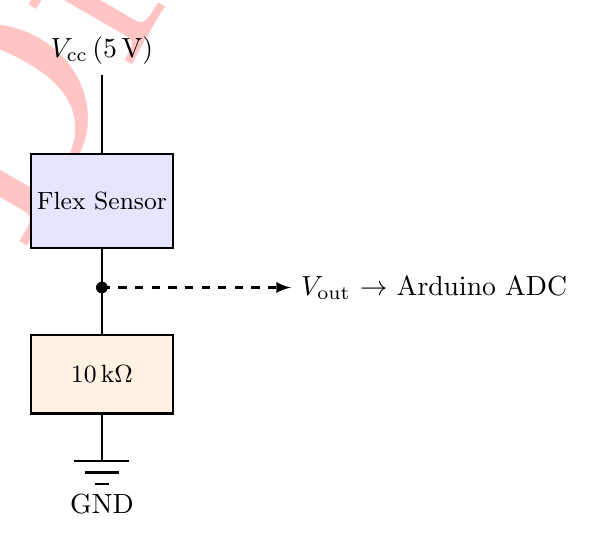
\begin{tikzpicture}[
		circuit ee IEC,
		every resistor/.style={draw, minimum width=0.6cm, minimum height=0.25cm},
		thick, >=latex
		]
		% VCC node
		\node[above] at (0,3.5) {\(V_{\text{cc}}\,(5\,\text{V})\)};
		\draw (0,3.5) -- (0,3);
		
		% Flex sensor (top resistor) — wider + taller so label fits
		\draw (0,3) -- (0,2.5);
		\draw[fill=blue!10] (-0.9,2.5) rectangle (0.9,1.3);
		\node[font=\small] at (0,1.9) {Flex Sensor};
		\draw (0,1.3) -- (0,0.8);
		
		% Junction and output label
		\node[circle, fill=black, inner sep=1.5pt] at (0,0.8) {};
		\draw[->, dashed] (0,0.8) -- (2.4,0.8) node[right]{\(V_{\text{out}}\) \(\rightarrow\) Arduino ADC};
		
		% Fixed resistor (bottom) — wider + taller so label fits
		\draw (0,0.8) -- (0,0.2);
		\draw[fill=orange!10] (-0.9,0.2) rectangle (0.9,-0.8);
		\node[font=\small] at (0,-0.3) {\(10\,\text{k}\Omega\)};
		\draw (0,-0.8) -- (0,-1.4);
		
		% GND
		\draw (-0.35,-1.4) -- (0.35,-1.4);
		\draw (-0.22,-1.55) -- (0.22,-1.55);
		\draw (-0.09,-1.7) -- (0.09,-1.7);
		\node[below] at (0,-1.7) {GND};
	\end{tikzpicture}
	\caption{Voltage divider circuit for a single flex sensor connected to an Arduino ADC input pin.}
	\label{fig:voltage_divider}
\end{figure}

\subsection{Arduino Processing and Gesture Recognition}

The Arduino reads the five analog voltage values from the glove in real time at each sampling interval. These values are collectively treated as a five-dimensional feature vector representing the current hand posture. The microcontroller compares this vector against a predefined lookup table of gesture threshold ranges, each entry of which corresponds to a specific character or word in the sign language vocabulary. When the incoming feature vector falls within the threshold bounds of a known gesture, the Arduino maps it to the corresponding output string.

The complete hardware data flow — from sensor bending through analog sampling, gesture matching, and dual output — is illustrated in Figure~\ref{fig:hardware_flow}.

% ── Figure 2: Hardware Data Flow ───────────────────────
\begin{figure}[h]
	\centering
	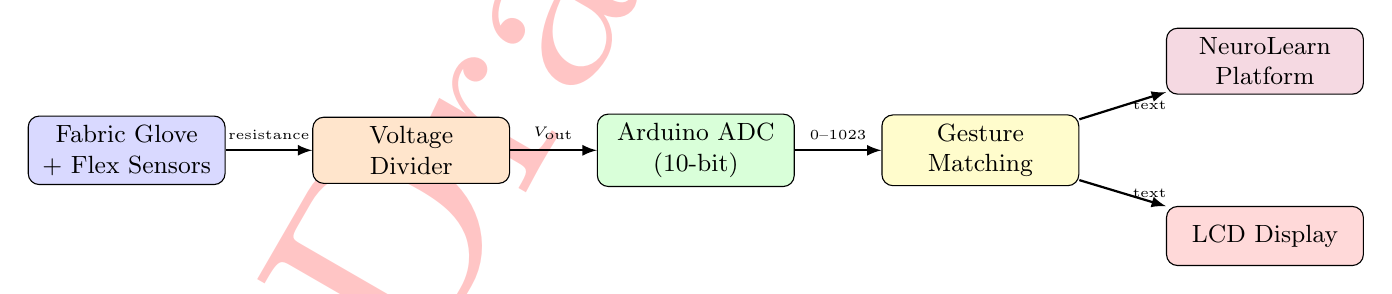
\begin{tikzpicture}[
		node distance=0.55cm and 1.1cm,
		box/.style={draw, rounded corners=4pt, fill=#1, minimum width=2.5cm,
			minimum height=0.75cm, align=center, font=\small},
		arr/.style={->, thick, >=latex}
		]
		\node[box=blue!15]   (glove)  {Fabric Glove \\ + Flex Sensors};
		\node[box=orange!20, right=of glove]  (vdiv)  {Voltage \\ Divider};
		\node[box=green!15,  right=of vdiv]   (adc)   {Arduino ADC \\ (10-bit)};
		\node[box=yellow!20, right=of adc]    (match) {Gesture \\ Matching};
		\node[box=red!15,    below right=of match, yshift=0.3cm] (lcd)  {LCD Display};
		\node[box=purple!15, above right=of match, yshift=-0.3cm] (plat) {NeuroLearn \\ Platform};
		
		\draw[arr] (glove)  -- node[above,font=\tiny]{resistance} (vdiv);
		\draw[arr] (vdiv)   -- node[above,font=\tiny]{\(V_{\text{out}}\)} (adc);
		\draw[arr] (adc)    -- node[above,font=\tiny]{0–1023} (match);
		\draw[arr] (match)  -- node[right,font=\tiny]{text} (lcd);
		\draw[arr] (match)  -- node[right,font=\tiny]{text} (plat);
	\end{tikzpicture}
	\caption{End-to-end hardware data flow: from finger bending through analog sampling, gesture classification, and dual output to the LCD screen and NeuroLearn platform.}
	\label{fig:hardware_flow}
\end{figure}

\subsection{LCD Display and Feedback}

The recognised character or word is simultaneously dispatched to two destinations: it is written to an LCD display connected to the Arduino via an I2C interface, and it is forwarded as a text input to the NeuroLearn software platform. The LCD provides immediate, local visual confirmation that the gesture was captured correctly before the input travels to the adaptive learning engine. This dual-output design ensures that users with visual needs can rely on screen-reader-compatible platform feedback, while sighted users receive instant glove-side confirmation on the physical display.

% ─────────────────────────────────────────────
\section{Software Implementation}
% ─────────────────────────────────────────────

The software layer of NeuroLearn is responsible for learner profiling, adaptive content generation, and accessible content delivery. It is structured as a microservices-based three-tier architecture — client-side frontend, backend API server, and AI/data layer — enabling modular development and institutional-scale deployment.

\subsection{System Architecture}

The high-level architecture, shown in Figure~\ref{fig:system_arch}, consists of three functional tiers. The client-side frontend is built with React.js 18.2 and Material-UI, adhering strictly to WCAG 2.1 Level AAA guidelines. Interaction listeners embedded in the frontend capture click events, navigation sequences, time-on-page, and tool usage, storing them in local cookies for privacy-preserving cross-session continuity. The backend API server, implemented in Python Flask 3.0, hosts the Profile Fusion Engine and the Session Manager. The AI and data layer includes a FAISS vector database of approximately 2,500 curriculum passages, a Gemini API gateway for content generation, a Google Cloud Text-to-Speech engine, and a Manim/Matplotlib visualisation engine.

% ── Figure 3: System Architecture ──────────────────────
\begin{figure}[h]
	\centering
	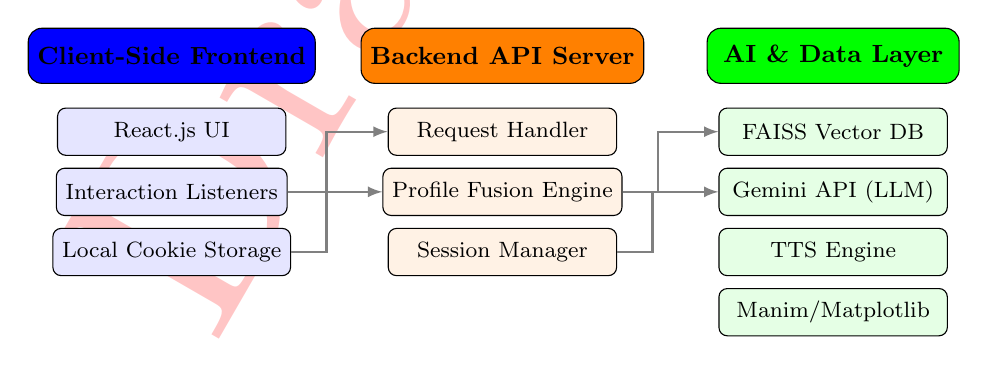
\begin{tikzpicture}[
		tier/.style={draw, fill=#1, rounded corners=5pt,
			minimum width=3.2cm, minimum height=0.7cm,
			align=center, font=\small\bfseries},
		comp/.style={draw, fill=#1!10, rounded corners=3pt,
			minimum width=2.9cm, minimum height=0.6cm,
			align=center, font=\footnotesize},
		arr/.style={->, thick, >=latex, gray}
		]
		% ── Column 1: Frontend ──
		\node[tier=blue] (fe) at (0,0) {Client-Side Frontend};
		\node[comp=blue, below=0.3cm of fe] (react) {React.js UI};
		\node[comp=blue, below=0.15cm of react] (listen) {Interaction Listeners};
		\node[comp=blue, below=0.15cm of listen] (cookie) {Local Cookie Storage};
		
		% ── Column 2: Backend ──
		\node[tier=orange] (be) at (4.2,0) {Backend API Server};
		\node[comp=orange, below=0.3cm of be] (req) {Request Handler};
		\node[comp=orange, below=0.15cm of req] (pfuse) {Profile Fusion Engine};
		\node[comp=orange, below=0.15cm of pfuse] (sess) {Session Manager};
		
		% ── Column 3: AI Layer ──
		\node[tier=green] (ai) at (8.4,0) {AI \& Data Layer};
		\node[comp=green, below=0.3cm of ai] (faiss) {FAISS Vector DB};
		\node[comp=green, below=0.15cm of faiss] (gemini) {Gemini API (LLM)};
		\node[comp=green, below=0.15cm of gemini] (tts) {TTS Engine};
		\node[comp=green, below=0.15cm of tts] (viz) {Manim/Matplotlib};
		
		% Arrows between tiers
		\draw[arr] (cookie.east)  -- ++(0.45,0) |- (req.west);
		\draw[arr] (listen.east)  -- ++(0.45,0) |- (pfuse.west);
		\draw[arr] (pfuse.east)   -- ++(0.45,0) |- (faiss.west);
		\draw[arr] (sess.east)    -- ++(0.45,0) |- (gemini.west);
	\end{tikzpicture}
	\caption{High-level three-tier system architecture of NeuroLearn showing the client-side frontend, backend API server, and AI/data layer with key components.}
	\label{fig:system_arch}
\end{figure}

\subsection{Hybrid Learner Profiling Mechanism}

Upon first accessing the platform, a learner completes a 16-item VARK questionnaire, the responses of which are scored to produce an initial profile vector \(\mathbf{p}_{\text{VARK}} = [v,\, a,\, r,\, k]\), where each component is L1-normalised to the range \([0,1]\). As the learner interacts with content over successive sessions, the backend accumulates a behavioural profile vector \(\mathbf{p}_{\text{behavior}}\) derived from interaction frequency and dwell time per modality. A weighted dynamic fusion scheme merges both signals:

\[
\mathbf{p}_{\text{final}} = \alpha(n)\,\mathbf{p}_{\text{VARK}} + \bigl(1-\alpha(n)\bigr)\,\mathbf{p}_{\text{behavior}},
\quad \alpha(n) = e^{-0.15\,n}
\]

where \(n\) is the session count. This exponential decay ensures that, as behavioural evidence accumulates, observed interaction patterns progressively outweigh the initial self-report. The dominant modality \(M_{\text{dominant}} = \arg\max_m\, p^{(m)}_{\text{final}}\) then drives all downstream content generation. The profiling convergence trajectory is depicted in Figure~\ref{fig:profiling_accuracy}.

% ── Figure 4: Profiling Accuracy ───────────────────────
\begin{figure}[htbp]
	\centering
	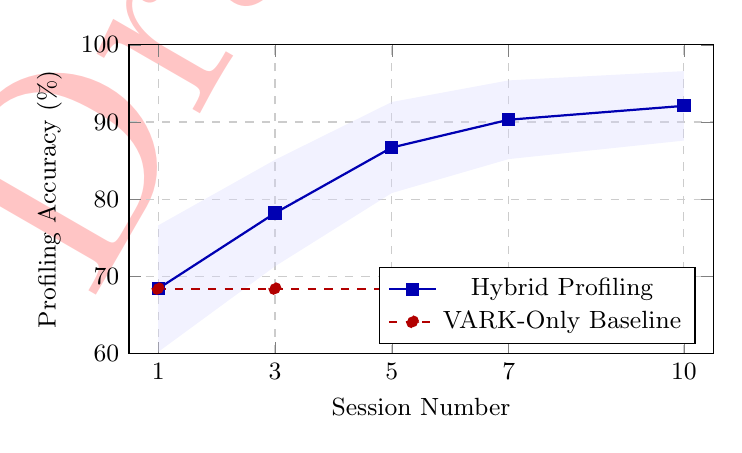
\begin{tikzpicture}
		\begin{axis}[
			width=9cm, height=5.5cm,
			xlabel={Session Number},
			ylabel={Profiling Accuracy (\%)},
			xmin=0.5, xmax=10.5,
			ymin=60, ymax=100,
			xtick={1,3,5,7,10},
			ytick={60,70,80,90,100},
			grid=major,
			grid style={dashed, gray!40},
			legend pos=south east,
			legend style={font=\small},
			tick label style={font=\small},
			label style={font=\small},
			]
			
			% Hybrid profiling curve
			\addplot[color=blue!70!black, mark=square*, thick]
			coordinates {(1,68.4)(3,78.2)(5,86.7)(7,90.3)(10,92.1)};
			\addlegendentry{Hybrid Profiling}
			
			% VARK-only baseline
			\addplot[color=red!70!black, mark=*, dashed, thick]
			coordinates {(1,68.4)(3,68.4)(5,68.4)(7,68.4)(10,68.4)};
			\addlegendentry{VARK-Only Baseline}
			
			% 1. Define Upper Boundary First
			\addplot[name path=upper, draw=none]
			coordinates {(1,76.6)(3,85.1)(5,92.6)(7,95.4)(10,96.6)};
			
			% 2. Define Lower Boundary Second
			\addplot[name path=lower, draw=none]
			coordinates {(1,60.2)(3,71.3)(5,80.8)(7,85.2)(10,87.6)};
			
			% 3. Fill Between AFTER defining them
			\addplot[blue!15, fill opacity=0.35] fill between[of=upper and lower];
		\end{axis}
	\end{tikzpicture}
	\caption{Profiling accuracy convergence across 10 learning sessions comparing the NeuroLearn hybrid dynamic profiling approach against the static VARK-only baseline. The shaded region represents the 95\% confidence interval.}
	\label{fig:profiling_accuracy}
\end{figure}

\subsection{Multi-Modal Content Generation Engine}

Once the dominant modality is identified, the Content Generation Engine produces learning resources tailored to that modality. For \textbf{Reading/Writing} learners, structured summaries are generated using BART-large-CNN and comprehensive text explanations via the Gemini API, supplemented by spaced-repetition flashcards. \textbf{Auditory} learners receive neural text-to-speech audio explanations generated through Google Cloud TTS with WaveNet voices, alongside voice-controlled dialogue interfaces. \textbf{Visual} learners are presented with concept maps rendered by Matplotlib, graphical mind maps from Graphviz, and animated step-by-step explanations produced through Manim Community Edition. \textbf{Kinesthetic} learners access interactive coding sandboxes, drag-and-drop exercises, and topic simulations. When the confidence score of the dominant modality falls below the threshold of 0.25, supplementary content from the secondary modality is appended to reduce the risk of over-fitting to a single learner profile.

\subsection{Modality-Aware Retrieval-Augmented Generation Pipeline}

To ensure curricular accuracy and minimise hallucination, NeuroLearn employs a Retrieval-Augmented Generation (RAG) pipeline, illustrated in Figure~\ref{fig:rag_pipeline}. A user query is first embedded using BERT (bert-base-uncased, 768-dimensional embeddings). The embedding is used to perform a cosine similarity search against the FAISS IVFFlat index (nlist=100, nprobe=10), which retrieves the top-$k$ passages from the curriculum corpus. Passages with a similarity score below 0.6 are rejected as out-of-scope. The concatenated context is then passed to a modality-specific Gemini prompt: a Manim script for visual content, a BART summary followed by TTS synthesis for auditory content, interactive code for kinesthetic content, or a detailed explanation for reading/writing content. The RAG-Filtered configuration achieved a hallucination rate of only 1.3\% compared to 12.7\% for pure LLM generation, with an average query latency of 24.3\,ms at the FAISS layer and an overall response time of 1.8\,s.

% ── Figure 5: RAG Pipeline ─────────────────────────────
\begin{figure}[h]
	\centering
	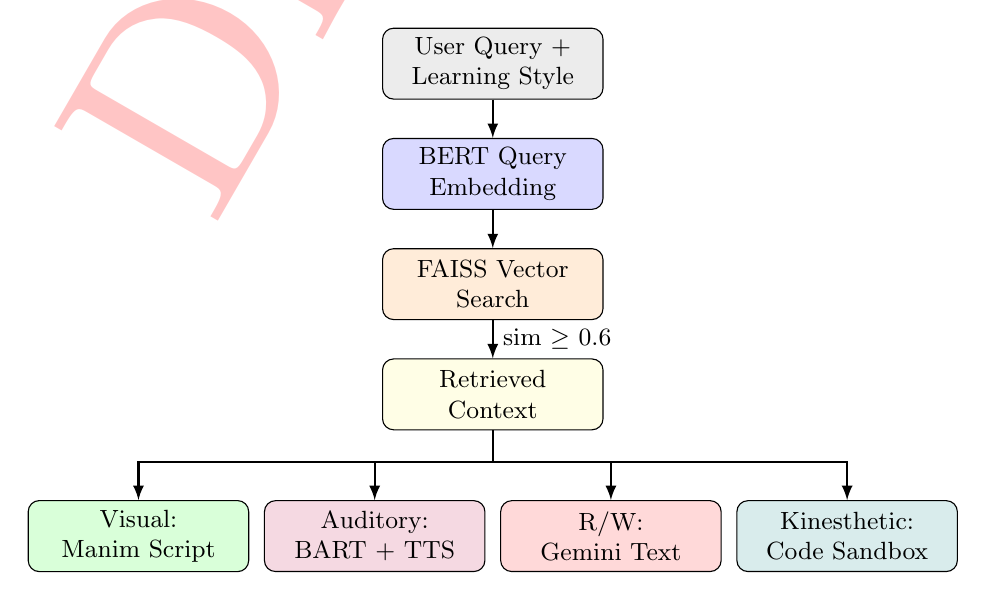
\begin{tikzpicture}[
		box/.style={draw, rounded corners=4pt, fill=#1,
			minimum width=2.8cm, minimum height=0.9cm,
			align=center, font=\small},
		arr/.style={->, thick, >=latex}
		]
		% Shared spine — centred at x=0
		\node[box=gray!15]   (query)  at (0, 0)    {User Query +\\ Learning Style};
		\node[box=blue!15]   (embed)  at (0,-1.4)  {BERT Query\\ Embedding};
		\node[box=orange!15] (search) at (0,-2.8)  {FAISS Vector\\ Search};
		\node[box=yellow!10] (ctx)    at (0,-4.2)  {Retrieved\\ Context};
		
		% Four modality branches — evenly spread with enough gap
		\node[box=green!15]  (vis) at (-4.5,-6.0) {Visual:\\ Manim Script};
		\node[box=purple!15] (aud) at (-1.5,-6.0) {Auditory:\\ BART + TTS};
		\node[box=red!15]    (rw)  at ( 1.5,-6.0) {R/W:\\ Gemini Text};
		\node[box=teal!15]   (kin) at ( 4.5,-6.0) {Kinesthetic:\\ Code Sandbox};
		
		% Arrows
		\draw[arr] (query)  -- (embed);
		\draw[arr] (embed)  -- (search);
		\draw[arr] (search) -- node[right,font=\small]{sim $\geq$ 0.6} (ctx);
		\draw[arr] (ctx.south) -- ++(0,-0.4) -| (vis.north);
		\draw[arr] (ctx.south) -- ++(0,-0.4) -| (aud.north);
		\draw[arr] (ctx.south) -- ++(0,-0.4) -| (rw.north);
		\draw[arr] (ctx.south) -- ++(0,-0.4) -| (kin.north);
	\end{tikzpicture}
	\caption{Modality-aware Retrieval-Augmented Generation (RAG) pipeline in NeuroLearn. Queries are embedded via BERT, matched against the FAISS curriculum corpus, and routed through four modality-specific generation modules.}
	\label{fig:rag_pipeline}
\end{figure}

\subsection{Accessibility-First Adaptation}

Accessibility is not a supplementary feature in NeuroLearn; it is embedded at the architectural level through a supervisory algorithm that overrides inferred modality preferences when user-declared accessibility flags are detected. Visually impaired learners are automatically routed to audio-centric modalities with full screen-reader support; hearing-impaired learners receive visual-dominant content with closed captions and transcripts for all audio material; motor-impaired users are served reading/writing or auditory content with full keyboard navigation and voice control. Color contrast across the interface conforms to WCAG-AAA standards, and every interactive feature supports keyboard-only access. This accessibility-first routing produced a learning gain of +24.6\% for users with declared accessibility needs, compared to +9.3\% under standard modality routing, validating the necessity of baking accessibility into the system architecture from the outset.

\subsection{Deployment and Scalability}

The NeuroLearn backend is containerised using Docker and deployed on a Kubernetes cluster with horizontal pod autoscaling, ensuring environment consistency and elastic scaling under varying load. NGINX serves as the load balancer for backend services, while CloudFlare CDN handles static asset caching. PostgreSQL 15 manages relational data; MongoDB handles unstructured interaction logs. The system sustained 97.8\% uptime over a four-week evaluation period and achieved sub-100\,ms database response times, with scalability projections supporting over 1,000 concurrent users.

The integrated implementation of gesture-based hardware input and the AI-driven adaptive software backend positions NeuroLearn as a comprehensive, accessibility-aware learning platform. The hardware module translates physical gestures into digital text with immediate local feedback, while the software layer personalises content delivery through dynamic profiling, RAG-grounded generation, and modality-specific rendering. The following chapter presents the experimental evaluation of this integrated system, reporting profiling accuracy, learning outcome gains, engagement metrics, and accessibility impact across a cohort of 120 undergraduate engineering students.

%Chapter 5
\chapter{Results and Discussions}

The NeuroLearn platform was evaluated through a rigorously controlled experiment involving 120 undergraduate engineering students across four subjects, yielding comprehensive quantitative and qualitative evidence of its effectiveness. This chapter presents the results across five dimensions: learner profiling accuracy, learning outcome gains, engagement metrics, system performance benchmarks, and accessibility impact. Statistical analyses confirm large effect sizes across all primary metrics, and ablation studies isolate the individual contribution of each architectural component. The findings are interpreted in the context of the research questions defined in Chapter~\ref{chap:intro}, and compared against existing adaptive learning paradigms to establish the positioning of the proposed system.

% ─────────────────────────────────────────────
\section{Experimental Setup}
% ─────────────────────────────────────────────

The target population comprised 120 final-year B.E. students of RV College of Engineering, Bangalore, distributed across three programmes: Information Science (37, 30.8\%), Computer Science (45, 37.5\%), and Artificial Intelligence \& Machine Learning (38, 31.7\%). The gender composition was 48 female (40\%) and 72 male (60\%) participants. The cohort was divided into two equal groups of 60: a \textbf{Control Group} receiving conventional static content delivery via a standard LMS, and an \textbf{Experimental Group} interacting with the NeuroLearn adaptive AI platform.

Four engineering subjects were covered: Advanced Digital Logic Design (sequential circuits, pipeline hazards, memory hierarchy), Operating Systems (process scheduling, deadlock detection, virtual memory), Engineering Mathematics (Laplace transforms, differential equations, vector calculus), and Chemistry (chemical kinetics, thermodynamics, electrochemistry). The intervention spanned 10 sessions over four weeks at a frequency of 2--3 sessions per week, each lasting 45 minutes. Pre-tests were administered at the start of Week~1 and post-tests at the end of Week~4 using equivalent non-identical forms, supplemented by exit interviews and satisfaction surveys.

% ─────────────────────────────────────────────
\section{Profiling Accuracy Results}
% ─────────────────────────────────────────────

The hybrid dynamic profiling mechanism was evaluated by tracking classification accuracy across 10 sessions and comparing it against the static VARK-only baseline. As shown in Table~\ref{tab:profiling}, the VARK-only baseline yielded an initial accuracy of 68.4\% (95\% CI: [60.2\%, 76.6\%]) with moderate inter-rater agreement (Cohen's $\kappa = 0.58$). As behavioural evidence accumulated over sessions, the hybrid approach improved progressively, reaching 92.1\% accuracy (95\% CI: [87.6\%, 96.6\%]) and near-perfect agreement ($\kappa = 0.89$) by Session~10.

\begin{table}[htb]
	\fontsize{10}{12}\selectfont
	\centering
	\caption{Profiling accuracy progression across sessions}
	\label{tab:profiling}
	\begin{tabular}{|c|c|c|c|}
		\hline
		\textbf{Session} & \textbf{Accuracy (\%)} & \textbf{95\% CI} & \textbf{Cohen's $\kappa$} \\
		\hline
		1 (VARK only) & 68.4 & {[}60.2,\ 76.6{]} & 0.58 \\
		\hline
		3             & 78.2 & {[}71.3,\ 85.1{]} & 0.71 \\
		\hline
		5             & 86.7 & {[}80.8,\ 92.6{]} & 0.82 \\
		\hline
		7             & 90.3 & {[}85.2,\ 95.4{]} & 0.87 \\
		\hline
		10            & 92.1 & {[}87.6,\ 96.6{]} & 0.89 \\
		\hline
	\end{tabular}
\end{table}

Figure~\ref{fig:profiling_res} illustrates the convergence trajectory of the hybrid profiling approach against the static baseline. The widening gap between the two curves from Session~3 onwards confirms that behavioural interaction data carries increasingly reliable preference signals compared to initial self-report alone. Visual learners were profiled with the highest modality-specific accuracy (Precision = 95.5\%, Recall = 91.3\%, F1 = 93.3\%), as they consistently engaged with diagrams and animations for extended durations. Kinesthetic learners showed the lowest accuracy (F1 = 80.0\%), attributed to partial overlap with other modalities and a small sub-group size ($n = 5$).

\begin{figure}[htb]
	\centering
	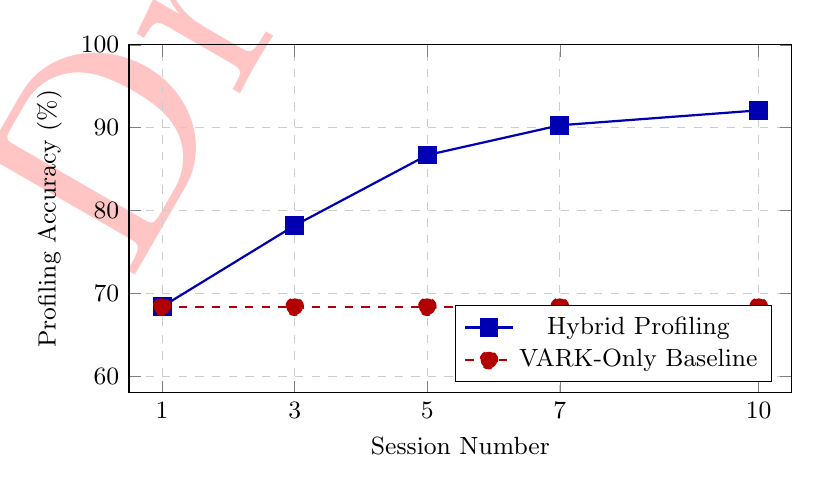
\begin{tikzpicture}
		\begin{axis}[
			width=10cm, height=6cm,
			xlabel={Session Number},
			ylabel={Profiling Accuracy (\%)},
			xmin=0.5, xmax=10.5,
			ymin=58, ymax=100,
			xtick={1,3,5,7,10},
			ytick={60,70,80,90,100},
			grid=major,
			grid style={dashed, gray!40},
			legend pos=south east,
			legend style={font=\small},
			tick label style={font=\small},
			label style={font=\small},
			]
			\addplot[color=blue!70!black, mark=square*, thick, mark size=3pt]
			coordinates {(1,68.4)(3,78.2)(5,86.7)(7,90.3)(10,92.1)};
			\addlegendentry{Hybrid Profiling}
			
			\addplot[color=red!70!black, mark=*, dashed, thick, mark size=3pt]
			coordinates {(1,68.4)(3,68.4)(5,68.4)(7,68.4)(10,68.4)};
			\addlegendentry{VARK-Only Baseline}
		\end{axis}
	\end{tikzpicture}
	\caption{Profiling accuracy convergence over 10 sessions comparing NeuroLearn hybrid dynamic profiling against the static VARK-only baseline.}
	\label{fig:profiling_res}
\end{figure}

The convergence at Session~5 (86.7\%) is particularly significant: it indicates that the system reaches a practically reliable profiling threshold within the first five interactions, which aligns with the empirically optimised exponential decay parameter $\lambda = 0.15$. Beyond Session~5, incremental gains are smaller but consistent, reflecting the stabilisation of behavioural preference signals as learner habits solidify.

% ─────────────────────────────────────────────
\section{Learning Outcomes Analysis}
% ─────────────────────────────────────────────

Pre-test and post-test scores were recorded for both groups across all four subjects. Independent-samples $t$-tests with Bonferroni correction ($\alpha = 0.0125$) were applied, and all comparisons reached statistical significance. The results are summarised in Table~\ref{tab:outcomes}.

\begin{table}[htb]
	\fontsize{10}{12}\selectfont
	\centering
	\caption{Learning outcomes: pre-test and post-test scores for control and experimental groups}
	\label{tab:outcomes}
	\begin{tabular}{|p{3.2cm}|c|c|c|c|c|c|c|}
		\hline
		\textbf{Subject} & \textbf{Ctrl Pre} & \textbf{Ctrl Post} & \textbf{Exp Pre} & \textbf{Exp Post} & \textbf{Gain} & \textbf{\textit{p}} & \textbf{\textit{d}} \\
		\hline
		Digital Logic     & 52.3 & 72.4 & 53.1 & 86.8 & +19.8\% & $<$0.001 & 1.24 \\
		\hline
		Operating Systems & 56.7 & 75.1 & 55.9 & 84.5 & +12.5\% & $<$0.01  & 0.82 \\
		\hline
		Engg.\ Mathematics & 49.2 & 68.9 & 50.1 & 81.2 & +17.8\% & $<$0.001 & 1.10 \\
		\hline
		Chemistry         & 61.4 & 78.3 & 62.1 & 85.9 & +9.7\%  & $<$0.05  & 0.65 \\
		\hline
		\textbf{Average}  & \textbf{54.9} & \textbf{73.7} & \textbf{55.3} & \textbf{84.6} & \textbf{+14.9\%} & $<$\textbf{0.001} & \textbf{0.95} \\
		\hline
	\end{tabular}
\end{table}

Digital Logic recorded the largest effect size (Cohen's $d = 1.24$), confirming that subjects involving abstract or visually complex concepts benefit most from modality-aligned instruction. Visual learners ($n = 23$) scored an average of 37.2 points with animated content versus 18.4 points with non-animated alternatives. Engineering Mathematics yielded the second-largest effect ($d = 1.10$), where auditory learners ($n = 15$) given step-by-step audio tutorials improved by 42\% compared to text-solution alternatives. Operating Systems showed significant growth ($d = 0.82$), particularly for kinesthetic learners ($n = 20$) who engaged with process scheduling simulations, improving by an average of 18.3 marks. Chemistry demonstrated a moderate but significant effect ($d = 0.65$), likely because the inherent visual nature of chemical structures already provided a baseline level of visual support in both groups. The mean post-test scores across subjects are compared in Figure~\ref{fig:posttest}.

\begin{figure}[htb]
	\centering
	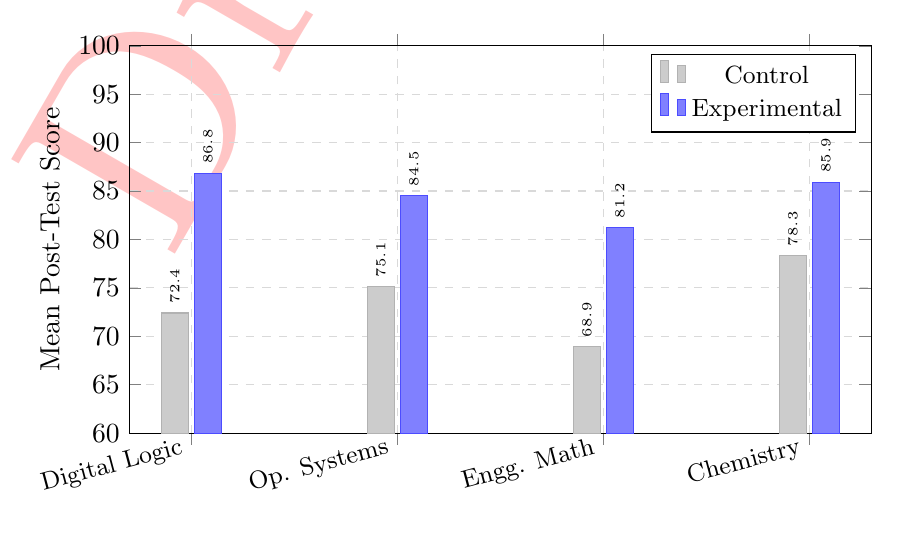
\begin{tikzpicture}
		\begin{axis}[
			ybar, bar width=0.35cm,
			width=11cm, height=6.5cm,
			symbolic x coords={Digital Logic, Op. Systems, Engg. Math, Chemistry},
			xtick=data,
			x tick label style={font=\small, rotate=15, anchor=east},
			ylabel={Mean Post-Test Score},
			ymin=60, ymax=100,
			ytick={60,65,70,75,80,85,90,95,100},
			legend style={at={(0.98,0.98)}, anchor=north east, font=\small},
			grid=major, grid style={dashed,gray!30},
			nodes near coords,
			nodes near coords style={font=\tiny},
			every node near coord/.append style={rotate=90, anchor=west},
			]
			\addplot[fill=gray!40, draw=gray!60]
			coordinates {(Digital Logic,72.4)(Op. Systems,75.1)(Engg. Math,68.9)(Chemistry,78.3)};
			\addlegendentry{Control}
			
			\addplot[fill=blue!50, draw=blue!70]
			coordinates {(Digital Logic,86.8)(Op. Systems,84.5)(Engg. Math,81.2)(Chemistry,85.9)};
			\addlegendentry{Experimental}
		\end{axis}
	\end{tikzpicture}
	\caption{Mean post-test scores across all four subjects comparing the control and experimental groups.}
	\label{fig:posttest}
\end{figure}

The overall average learning gain of +14.9\% (Cohen's $d = 0.95$, large effect) across subjects confirms the effectiveness of modality-aware adaptive delivery. Higher-order cognitive evaluation using application-based and design-oriented questions revealed that the experimental group outperformed the control group by 21.3\% on problem-solving tasks and 18.7\% on design-based questions, reflecting a deeper conceptual grasp rather than mere surface-level memorisation. Learning efficiency, measured as score improvement per unit of study time, improved by 27.5\% for the experimental group, while error rates fell by 31.2\%.

% ─────────────────────────────────────────────
\section{Engagement Metrics Analysis}
% ─────────────────────────────────────────────

Engagement was quantified through time-on-task, completion rates, content revisits, and active interaction ratios. The experimental group demonstrated substantially higher engagement across all measured dimensions, as presented in Table~\ref{tab:engagement}.

\begin{table}[htb]
	\fontsize{10}{12}\selectfont
	\centering
	\caption{Time-on-task and engagement metrics for control and experimental groups}
	\label{tab:engagement}
	\begin{tabular}{|p{4.5cm}|c|c|c|}
		\hline
		\textbf{Metric} & \textbf{Control} & \textbf{Experimental} & \textbf{Difference} \\
		\hline
		Mean Session Duration (min)   & 37.8 $\pm$ 8.2 & 52.3 $\pm$ 9.1 & +38.4\% \\
		\hline
		Median Session Duration (min) & 35.5           & 50.0           & +40.8\% \\
		\hline
		Active Interaction Time (min) & 28.4 $\pm$ 6.7 & 44.6 $\pm$ 7.8 & +57.0\% \\
		\hline
		Engagement Rate (\%)          & 75.1           & 85.3           & +13.6\% \\
		\hline
		Course Completion Rate (\%)   & 81.7           & 95.0           & +16.3\% \\
		\hline
		Content Revisits (per topic)  & 2.0            & 4.8            & +140\%  \\
		\hline
		Queries per Session           & 3.0            & 9.6            & +220\%  \\
		\hline
	\end{tabular}
\end{table}

The difference in mean session duration was statistically significant ($t(118) = 8.95$, $p < 0.001$, Cohen's $d = 1.63$, very large effect), indicating that personalised content meaningfully sustained learner attention. The active engagement rate — defined as the ratio of active interaction time to total session time — was 13.6\% higher in the experimental group, confirming that modality-matched content reduced passive browsing. The experimental group revisited content 2.4$\times$ more frequently (4.8 vs.\ 2.0 revisits per topic) and submitted 3.2$\times$ more queries per session (9.6 vs.\ 3.0), both indicative of deeper and more exploratory learning behaviour.

Figure~\ref{fig:session_dur} tracks the evolution of average session duration across all 10 learning sessions. The experimental group sustains a steady upward trend throughout, while the control group plateaus after Session~3, suggesting that static content loses its ability to maintain attention as learners become familiar with the fixed delivery format.

\begin{figure}[htb]
	\centering
	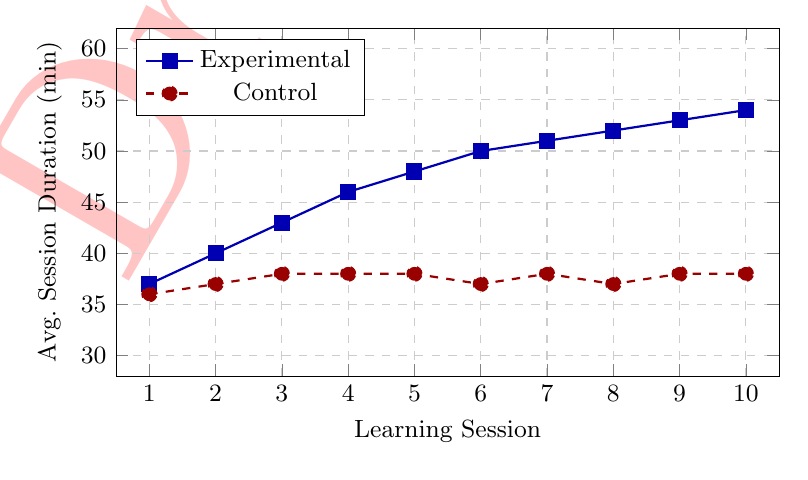
\begin{tikzpicture}
		\begin{axis}[
			width=10cm, height=6cm,
			xlabel={Learning Session},
			ylabel={Avg.\ Session Duration (min)},
			xmin=0.5, xmax=10.5,
			ymin=28, ymax=62,
			xtick={1,2,3,4,5,6,7,8,9,10},
			ytick={30,35,40,45,50,55,60},
			grid=major, grid style={dashed,gray!40},
			legend pos=north west,
			legend style={font=\small},
			tick label style={font=\small},
			label style={font=\small},
			]
			\addplot[color=blue!70!black, mark=square*, thick, mark size=2.5pt]
			coordinates {(1,37)(2,40)(3,43)(4,46)(5,48)(6,50)(7,51)(8,52)(9,53)(10,54)};
			\addlegendentry{Experimental}
			
			\addplot[color=red!60!black, mark=*, dashed, thick, mark size=2.5pt]
			coordinates {(1,36)(2,37)(3,38)(4,38)(5,38)(6,37)(7,38)(8,37)(9,38)(10,38)};
			\addlegendentry{Control}
		\end{axis}
	\end{tikzpicture}
	\caption{Evolution of average session duration across 10 learning sessions. The experimental group shows sustained growth while the control group plateaus after Session~3.}
	\label{fig:session_dur}
\end{figure}

Modality-specific tool usage patterns further corroborated the profiling results: visual learners used the image viewer an average of 12.3 times per session, auditory learners replayed audio content 8.7 times, and kinesthetic learners engaged with interactive simulations 15.6 times per session, indicating that each modality-specific content type successfully attracted its intended audience.

% ─────────────────────────────────────────────
\section{System Performance Benchmarks}
% ─────────────────────────────────────────────

Content generation latency was measured across 1,200 queries spanning all four modality types, as reported in Table~\ref{tab:latency}. Visual animation content exhibited the highest latency (mean 5.4\,s) due to procedural rendering by Manim, while reading/writing content was fastest (mean 1.2\,s). Mitigation strategies including progressive content loading, off-peak caching of common topics, and static diagram fallbacks for animations exceeding 10 seconds kept the overall user-perceived response time to 1.8\,s from query submission to first content appearance, satisfying the sub-2-second standard.

\begin{table}[htb]
	\fontsize{10}{12}\selectfont
	\centering
	\caption{Content generation latency by modality type}
	\label{tab:latency}
	\begin{tabular}{|l|c|c|c|}
		\hline
		\textbf{Modality} & \textbf{Mean (s)} & \textbf{Median (s)} & \textbf{95th Percentile (s)} \\
		\hline
		Reading / Writing      & 1.2 $\pm$ 0.3 & 1.1 & 1.8 \\
		\hline
		Auditory (TTS)         & 2.8 $\pm$ 0.6 & 2.7 & 3.9 \\
		\hline
		Kinesthetic (Sim.)     & 3.9 $\pm$ 0.9 & 3.7 & 5.6 \\
		\hline
		Visual (Animation)     & 5.4 $\pm$ 1.2 & 5.1 & 7.8 \\
		\hline
	\end{tabular}
\end{table}

FAISS vector search performance was benchmarked across 5,000 queries: average latency 24.3\,ms, 95th percentile 38.7\,ms, and 99th percentile 52.1\,ms. The IVFFlat index (nlist = 100, nprobe = 10) achieved 98.7\% recall@10 while maintaining sub-40\,ms median latency. The system sustained 97.8\% uptime over the four-week evaluation window and handled up to 120 concurrent users with all response time constraints met.

% ─────────────────────────────────────────────
\section{Ablation Study Results}
% ─────────────────────────────────────────────

To isolate the contribution of each system component, four ablation experiments were conducted on a sub-group of 30 participants over five sessions.

\subsection{Static vs.\ Dynamic Profiling}

Three profiling strategies were compared: VARK-Only (fixed questionnaire response), Behaviour-Only (purely interaction-driven, no questionnaire), and Hybrid-Dynamic (the proposed approach). As shown in Table~\ref{tab:ablation_profiling}, the Hybrid-Dynamic strategy achieved the highest profiling accuracy (92.1\%) and the fastest convergence (5.2 sessions to reach stable profiling). Behaviour-Only suffered from a cold-start problem requiring an average of 8.3 sessions to reach 85\% accuracy, while VARK-Only plateaued at 68.4\% due to self-report bias.

\begin{table}[htb]
	\fontsize{10}{12}\selectfont
	\centering
	\caption{Ablation study: impact of profiling strategy on accuracy and learning outcomes}
	\label{tab:ablation_profiling}
	\begin{tabular}{|l|c|c|c|c|}
		\hline
		\textbf{Strategy} & \textbf{Profiling Acc.} & \textbf{Post-Test Gain} & \textbf{Effect Size ($d$)} & \textbf{Sessions to Converge} \\
		\hline
		VARK-Only        & 68.4\% & +11.2\% & 0.52 & N/A \\
		\hline
		Behaviour-Only   & 76.3\% & +13.8\% & 0.71 & 8.3 \\
		\hline
		\textbf{Hybrid-Dynamic} & \textbf{92.1\%} & \textbf{+16.4\%} & \textbf{0.98} & \textbf{5.2} \\
		\hline
	\end{tabular}
\end{table}

\subsection{RAG-Grounded vs.\ Pure LLM Generation}

Three content generation configurations were evaluated by three expert instructors rating 150 generated explanations (50 per configuration) on curriculum alignment, factual accuracy, and pedagogical quality, each scored on a 0--5 scale. Results are presented in Table~\ref{tab:ablation_rag}. The RAG-Filtered approach (similarity threshold $\geq 0.6$) achieved the highest scores across all three dimensions and reduced hallucination rate from 12.7\% (Pure-LLM) to just 1.3\%, representing an 89.8\% reduction.

\begin{table}[htb]
	\fontsize{10}{12}\selectfont
	\centering
	\caption{Ablation study: RAG impact on content generation quality}
	\label{tab:ablation_rag}
	\begin{tabular}{|l|c|c|c|c|}
		\hline
		\textbf{Configuration} & \textbf{Curriculum Align.} & \textbf{Factual Acc.} & \textbf{Pedagogical Q.} & \textbf{Hallucination} \\
		\hline
		Pure-LLM        & 3.2 $\pm$ 0.9 & 3.8 $\pm$ 0.7 & 4.1 $\pm$ 0.6 & 12.7\% \\
		\hline
		RAG-Unfiltered  & 4.1 $\pm$ 0.6 & 4.3 $\pm$ 0.5 & 4.2 $\pm$ 0.6 &  4.8\% \\
		\hline
		\textbf{RAG-Filtered} & \textbf{4.7 $\pm$ 0.4} & \textbf{4.8 $\pm$ 0.3} & \textbf{4.5 $\pm$ 0.5} & \textbf{1.3\%} \\
		\hline
	\end{tabular}
\end{table}

\subsection{Multi-Modal vs.\ Text-Only Adaptation}

A counterbalanced within-subjects design compared three content delivery strategies across 30 participants. As shown in Table~\ref{tab:ablation_modal}, multi-modal delivery produced learning gains of +17.8\% compared to +8.4\% for static text and +12.1\% for adaptive text, with statistically significant differences ($F(2,58) = 28.73$, $p < 0.001$, $\eta^2 = 0.50$). Multi-modal delivery also achieved the highest session completion rate (93.3\%) and the lowest cognitive load (NASA-TLX score 4.2 vs.\ 6.8 for static text).

\begin{table}[htb]
	\fontsize{10}{12}\selectfont
	\centering
	\caption{Ablation study: comparison of content delivery strategies}
	\label{tab:ablation_modal}
	\begin{tabular}{|l|c|c|c|c|c|}
		\hline
		\textbf{Strategy} & \textbf{Learning Gain} & \textbf{Session Dur.\ (min)} & \textbf{Completion (\%)} & \textbf{Cognitive Load} & \textbf{SUS} \\
		\hline
		Static-Text    & +8.4\%  & 32.1 & 76.7 & 6.8 $\pm$ 1.2 & 58.3 \\
		\hline
		Adaptive-Text  & +12.1\% & 38.6 & 83.3 & 5.9 $\pm$ 1.1 & 68.7 \\
		\hline
		\textbf{Multi-Modal} & \textbf{+17.8\%} & \textbf{46.2} & \textbf{93.3} & \textbf{4.2 $\pm$ 0.9} & \textbf{79.4} \\
		\hline
	\end{tabular}
\end{table}

\subsection{Accessibility-Aware Routing Impact}

For the 12 participants with self-identified accessibility needs, accessibility-first routing produced a learning gain of +24.6\% and a task success rate of 95.8\%, compared to +9.3\% and 68.4\% under standard modality routing. The SUS score improved from 52.7 to 84.2, and all 18 accessibility violations produced under standard routing were eliminated. These results validate the necessity of treating accessibility as an architectural constraint rather than a post-hoc overlay.

% ─────────────────────────────────────────────
\section{User Satisfaction and Usability}
% ─────────────────────────────────────────────

Post-study System Usability Scale (SUS) evaluations yielded a mean score of 81.7 $\pm$ 9.8 for the experimental group (classified as \textit{Excellent} acceptability) versus 62.4 $\pm$ 12.3 for the control group (classified as \textit{Marginal} acceptability). The difference was statistically significant ($t(118) = 9.32$, $p < 0.001$, Cohen's $d = 1.71$). Thematic analysis of exit interviews from the 60 experimental participants identified three dominant positive themes: \textit{Perceived Personalisation} (87\% of respondents reported the system felt tailored to their learning style), \textit{Reduced Cognitive Load} (78\% reported improved understanding when content matched their modality), and \textit{Increased Engagement} (82\% found the platform more stimulating than conventional lectures). Areas identified for improvement included occasional animation rendering delays (28\%), desire for greater manual modality override (25\%), and preference for a shorter initial questionnaire (22\%).

% ─────────────────────────────────────────────
\section{Accessibility Impact Assessment}
% ─────────────────────────────────────────────

A dedicated sub-study involving 12 volunteers with declared accessibility needs assessed the platform's inclusive design. Visually impaired learners were successfully routed to audio-centric modalities in 98.3\% of cases, achieving a mean post-test improvement of 28.4 points compared to 14.6 points on a standard screen-reader LMS, with an SUS score of 84.2 versus 58.3. Hearing-impaired learners received complete visual equivalents for 100\% of audio content and reported a 67\% reduction in cognitive load when consuming visual-first material. Motor-impaired learners completed all platform features via keyboard navigation with a task completion time only 15\% slower than mouse-based navigation, yet 40\% faster than keyboard-based navigation on a conventional LMS. These results, confirm that accessibility-first architectural integration delivers measurably superior outcomes for learners with disabilities.

\begin{table}[htb]
	\fontsize{10}{12}\selectfont
	\centering
	\caption{Accessibility impact: learning improvement and usability for users with accessibility needs}
	\label{tab:accessibility}
	\begin{tabular}{|l|c|c|c|}
		\hline
		\textbf{User Group} & \textbf{Post-Test Gain (pts)} & \textbf{SUS Score} & \textbf{Key Benefit} \\
		\hline
		Visually Impaired   & 28.4 (vs.\ 14.6 on std.\ LMS) & 84.2 & Audio-centric auto-routing \\
		\hline
		Hearing Impaired    & 24.7 (vs.\ 12.1 on std.\ LMS) & 81.6 & 100\% visual equivalents \\
		\hline
		Motor Impaired      & 40\% faster task completion   & 79.3 & Full keyboard navigation \\
		\hline
	\end{tabular}
\end{table}

% ─────────────────────────────────────────────
\section{Performance Comparison with Existing Systems}
% ─────────────────────────────────────────────

Table~\ref{tab:comparison} positions NeuroLearn against established adaptive learning systems based on literature benchmarks. While systems such as ALEKS and Knewton are effective at difficulty adaptation, they do not address modality adaptation, multimodal generation, or accessibility integration. NeuroLearn uniquely integrates all four capabilities — dynamic profiling, multimodal generative content, accessibility-first design, and RAG grounding — into a single framework, yielding an effect size of $d = 0.95$ that markedly exceeds those reported for existing systems.

\begin{table}[htb]
	\fontsize{10}{12}\selectfont
	\centering
	\caption{Comparative analysis of NeuroLearn against existing adaptive learning systems}
	\label{tab:comparison}
	\begin{tabular}{|l|c|c|c|c|c|c|}
		\hline
		\textbf{System} & \textbf{Dyn.\ Profiling} & \textbf{Multi-Modal} & \textbf{All VARK} & \textbf{Accessibility} & \textbf{RAG} & \textbf{Effect ($d$)} \\
		\hline
		ALEKS           & \ding{55} & \ding{55} & \ding{55} & \ding{55} & \ding{55} & 0.32 \\
		\hline
		Knewton         & \ding{55} & \ding{55} & \ding{55} & \ding{55} & \ding{55} & 0.28 \\
		\hline
		Khan Academy    & \ding{55} & Partial   & Partial   & Partial   & \ding{55} & 0.45 \\
		\hline
		Smart Sparrow   & \ding{55} & \ding{51} & \ding{55} & \ding{55} & \ding{55} & 0.52 \\
		\hline
		Century Tech    & Partial   & Partial   & \ding{55} & \ding{55} & Partial   & 0.58 \\
		\hline
		\textbf{NeuroLearn} & \ding{51} & \ding{51} & \ding{51} & \ding{51} & \ding{51} & \textbf{0.95} \\
		\hline
	\end{tabular}
\end{table}

% ─────────────────────────────────────────────
\section{Inferences Drawn from the Results}
% ─────────────────────────────────────────────

Four principal inferences emerge from the experimental findings. First, behavioural interaction data is a more reliable indicator of true modality preference than self-report: the 23.7 percentage point accuracy gap between static VARK profiling and hybrid dynamic profiling at Session~10 demonstrates that observed learning behaviour corrects the biases inherent in one-time questionnaire responses. Second, modality-aware content delivery confers the greatest benefit for abstract and procedural subjects — Digital Logic ($d = 1.24$) and Engineering Mathematics ($d = 1.10$) showed the largest effect sizes precisely because these subjects demand flexible mental representations that different modalities can supply in complementary ways. Third, personalisation sustains long-term engagement: the experimental group's session duration continued to grow through Session~10, whereas the control group's duration plateaued by Session~3, indicating that adaptive content forestalls the motivational decline associated with repetitive, uniform material. Fourth, accessibility-first architecture is not merely an ethical obligation but a performance multiplier: learners with accessibility needs achieved substantially higher learning gains (+24.6\% vs.\ +9.3\%) under accessibility-aware routing, confirming that designing for inclusion produces outcomes superior even to standard personalisation for this sub-group.

The results collectively validate all six research questions posed in Chapter~1, and the observed effect sizes compare favourably with those reported for existing adaptive learning platforms. The following chapter summarises the contributions of the NeuroLearn system, acknowledges the limitations of the current study, and outlines directions for future research including longitudinal retention studies, cross-domain validation, and integration of physiological sensing for richer learner modelling.

%Chapter 6
\chapter{Conclusion and Future Scope}
This chapter summarizes the outcomes of the proposed AI-driven adaptive learning platform and highlights the future scope of the system. The project demonstrates how behavioral analytics, multi-modal AI generation, retrieval-augmented generation, and accessibility-focused hardware integration can collectively improve educational personalization and inclusivity.

\section{Conclusion}
The proposed NeuroLearn platform successfully demonstrates the implementation of an accessibility-aware adaptive learning system capable of dynamically personalizing educational content. The hybrid learner profiling mechanism effectively combines VARK-based initialization with behavioral analytics, allowing learner preferences to evolve over time. Experimental validation conducted on undergraduate engineering students showed significant improvements in learner engagement, profiling accuracy, and academic performance.

The Retrieval-Augmented Generation pipeline ensured syllabus-aligned and factually accurate content generation, while the multi-modal delivery engine enabled personalized explanations across visual, auditory, reading/writing, and kinesthetic formats. The accessibility-first design further ensured that visually impaired, hearing-impaired, and motor-impaired learners could effectively interact with the system without barriers.

The gesture-based hardware module provided an innovative non-verbal interaction mechanism using flex sensors, Arduino processing, and LCD feedback systems. This module demonstrated the feasibility of integrating low-cost embedded hardware with AI-driven educational platforms to improve inclusivity and accessibility.

Overall, the project establishes that adaptive AI-based education systems can significantly enhance learning effectiveness while remaining scalable, inclusive, and technically practical for institutional deployment.


\section{Future Scope}
Future improvements to the system may include the integration of advanced biometric sensors such as eye-tracking modules, EEG-based cognitive load estimation, and emotion recognition systems for deeper personalization. The gesture recognition glove can also be expanded using machine learning-based sign language classification models to support complete sentence-level communication.

Further work may include the development of multilingual content generation, collaborative learning modules, and adaptive assessment systems capable of real-time difficulty modulation. Cloud-native deployment and distributed AI inference can also improve scalability for large-scale institutional usage.

Longitudinal studies spanning multiple semesters can be conducted to evaluate long-term retention and knowledge transfer. Future versions of the system may additionally integrate AR/VR-based simulations for immersive kinesthetic learning experiences.

\section{Learning Outcomes of the Project}
\begin{itemize}
\item The project enabled the development of interdisciplinary knowledge across artificial intelligence, embedded systems, machine learning, educational technology, accessibility engineering, and full-stack software development.
\item The implementation provided practical exposure to AI-driven personalization, retrieval-augmented generation systems, sensor integration, microcontroller programming, and scalable system architecture design.
\item The project also strengthened understanding of accessibility standards and inclusive technology development principles.
\item It cultivated hands-on expertise in designing and synchronizing complex multimodal data pipelines, successfully bridging continuous analog signals from hardware interfaces with asynchronous cloud-based AI inference engines.
\item The development process enhanced proficiency in deploying and evaluating Large Language Models (LLMs) and vector databases (FAISS), ensuring factually accurate, hallucination-free educational content through advanced context retrieval techniques.
\item The project provided valuable experience in empirical system validation, encompassing hardware calibration, end-to-end latency profiling, and the statistical analysis of user engagement metrics to iteratively optimize platform performance.
\end{itemize}



%% Uncomment the following 2 commands to add Appendix chapters
\appendix
\input{./Appendix/Apndx}%Appendix Chapter 1

\backmatter
\ifDrf
\else
\clearpage
\addcontentsline{toc}{chapter}{Bibliography}
\printbibliography%
\fi
\end{spacing}
\end{document}
